\documentclass[letterpaper]{article} % DO NOT CHANGE THIS
% AAAI-27 Author Kit (official, https://aaai.org/authorkit27/, AuthorKit27.zip, aaai2027.sty dated 2026-10-21).
% AAAI anonymous workshop manuscript.
\usepackage[submission]{aaai2027}  % DO NOT CHANGE THIS
\usepackage[hyphens]{url}  % DO NOT CHANGE THIS
\usepackage{graphicx} % DO NOT CHANGE THIS
\urlstyle{rm} % DO NOT CHANGE THIS
\def\UrlFont{\rm}  % DO NOT CHANGE THIS
\usepackage{natbib}  % DO NOT CHANGE THIS AND DO NOT ADD ANY OPTIONS TO IT
\usepackage{caption} % DO NOT CHANGE THIS AND DO NOT ADD ANY OPTIONS TO IT
\frenchspacing  % DO NOT CHANGE THIS
\usepackage{algorithm}
\usepackage{algorithmic}
\usepackage{booktabs}
\usepackage{array}
\usepackage{amsmath}
\usepackage{placeins} % \FloatBarrier keeps appendix floats in their sections
\pdfinfo{
/TemplateVersion (2027.1)
}
\setcounter{secnumdepth}{2} % Section numbers enabled (permitted by the template: 0, 1 or 2).

\title{BrickForma: Crystallizing LLM Geometric Knowledge\\into Small Models for Text-to-Brick Assembly}
\author{Anonymous submission}
\affiliations{}

% AAAI sets \@maketitle in the full-width first-page title block.
% Append the teaser inside that block so it precedes the two-column abstract.
\AddToHook{cmd/@maketitle/after}{\par
\begingroup
\centering
% The standalone PDF already supplies a transparency group for its PNG tiles.
\pdfximage width \textwidth {figure1.pdf}%
\pdfrefximage\pdflastximage\par
\captionof{figure}{BrickForma overview. (a) Voxel-to-LEGO conversion. (b) Connectivity refinement. (c) Each triplet shows, from left to right, a voxel model from an LLM-authored generator, the LEGO assembly tiled from it, and a same-category BrickForma output (fine-tuned Qwen3-1.7B). Brick-type colors are for display only and are excluded from training targets.}
\label{fig:teaser}
\par
\endgroup
}

\begin{document}
\maketitle
\begin{abstract}
Geometric spatial reasoning underlies applications from robotics to automated design, yet the ability of large language models (LLMs) to turn a verbal description into a physically connected three-dimensional assembly remains largely underexplored. Brick assembly is a demanding constructive probe of this ability: a short, underspecified prompt leaves dimensions, proportions, and part layout implicit, and a valid answer must match the semantic intent of the prompt while completing this geometry with discrete pieces that interlock through studs. We study this setting as the \texttt{Text-to-Brick} task and present BrickForma, a framework that crystallizes the geometric knowledge of large language models into a compact model for this task. Parametric programs written with large language model assistance generate 80,000 source voxel models across 21 categories on a $48^3$ grid, each described at five levels of detail, yielding approximately 400,000 caption records that tie varying amounts of language to shared geometry. A voxel-to-brick conversion pipeline with connection analysis and local refinement turns these shapes into geometrically checked brick targets, on which we fine-tune Qwen3-1.7B with low-rank adaptation to predict brick dimensions and positions from text. A mixed-integer linear programming stage then seeks an exact cover of the voxel target reconstructed from these predictions with a single stud-connected component. On 525 shared prompts spanning five description levels, BrickForma's raw outputs achieve the highest mean VQAScore, PE, and SigLIP2 at every level among the three systems. BrickForma has a mean invalid-placement ratio of 0.79\%, compared with 0.00\% for BrickGPT and 18.42\% for BrickNet. These results suggest that executable programs and checked geometric data are an effective route for carrying spatial knowledge from large models into small models without the need of human-verified input for training.
\end{abstract}

% Reframed abstract and introduction for BrickForma.
% Result statements reflect the November 17 matched evaluation.
% New citation keys to add to the .bib: legopuzzles (Tang et al., 2025, arXiv:2503.19990),
% pfp (Zhou et al., AAAI 2026, Paper Folding Puzzles), geogrambench (Luo et al., ICLR 2026).




\section{Introduction}
Spatial reasoning and geometric understanding are fundamental to human cognition and to artificial intelligence, supporting applications from robotics and navigation to computer-aided design.
As large language models (LLMs) have matured, a growing body of work asks whether they can reason about shape, position, and transformation. Recent benchmarks probe LLMs' ability through 
%multi-step LEGO assembly~\cite{brickgpt, bricknet},
paper folding and unfolding~\cite{zhou2026paperfoldingpuzzle} and geometry expressed as procedural drawing code~\cite{luo2026geogrambench}. Each reports pronounced deficiencies in current models. These studies largely assess spatial reasoning by asking a model to select or compute an answer. A complementary and less examined question is whether a language model can \emph{construct}: given only words, can it produce a three-dimensional object whose parts are correctly sized, correctly placed, and physically joined?

%xiao: use lego instead of Brick
Lego brick assembly makes this question concrete. A concise narrative request such as \emph{a simple chair} identifies an object category while leaving its dimensions, proportions, and part layout largely unspecified. Answering it requires three coupled forms of geometric spatial reasoning. The model must complete the missing geometry from prior knowledge of what the object looks like. It must discretize that geometry into pieces of fixed dimensions at integer positions on a grid. And it must respect the difference between spatial adjacency and stud connectivity, since pieces that touch side by side do not hold together unless they interlock vertically through studs. We refer to this setting as the \texttt{Text-to-Brick} task: the translation from a natural-language description, at any level of detail, to a set of (Lego) brick placements that reproduces the described shape as a single connected assembly. Because every output can be checked for coverage, bounds, and connectivity, the task provides a verifiable test of whether linguistic knowledge has become spatial structure.

Prior work has established that language models can be trained for this task. BrickGPT~\cite{brickgpt} learns autoregressive brick-placement sequences and incorporates validity checks with physics-aware rollback during inference. BrickNet~\cite{bricknet} adopts a graph-based representation supporting a broader range of parts and connection types. Two questions remain open alongside these advances. \textbf{(Q1)} How well do generators translate \emph{limited} linguistic information into object geometry? In our five-level benchmark (Table~\ref{tab:level-results}), BrickNet obtains lower mean VQAScore, PE, and SigLIP2 than BrickForma at the two shortest description levels, L1 and L2, a gap that only level-wise evaluation makes visible. \textbf{(Q2)} Where should the geometric knowledge needed to answer concise requests come from? Large models hold broad knowledge of object proportions and part structure, but that knowledge is implicit and their outputs carry no structural guarantee. Whether it can be transferred to a compact model in a form that can be inspected and checked has received limited attention.

We present BrickForma, which addresses both questions by \emph{crystallizing} large-model geometric knowledge into a small model through executable programs rather than through the large model's direct outputs. With GPT-6.1 Sol assistance, we develop parametric programs that vary object proportions, part dimensions, openings, and support arrangements to synthesize voxel shapes in batches.
In this form, what a large model knows about a category becomes explicit and executable: each program fixes the structure of an object family and exposes its geometric degrees of freedom as parameters, so every generated shape is exact by construction. The source collection contains 80,000 models across 21 categories on a $48^3$ grid. Each model is paired with five levels of description that progressively introduce structural, geometric, proportional, and appearance information. The resulting approximately 400,000 caption records link concise requests and detailed specifications to shared geometry, so that a model trained on them learns to supply at the shortest level the geometric details that the longest level states outright.

Turning voxel shapes into brick targets is where spatial adjacency and stud connectivity must be separated. A connected voxel volume can be tiled by pieces that touch side by side without connecting through studs. Our conversion pipeline combines same-color tiling, connection analysis, and local refinement to construct geometrically checked target layouts, with changes to source voxels recorded in derived models. The integrated dataset release includes 79,301 models passing its dataset-level geometric checks. We fine-tune Qwen3-1.7B~\cite{qwen3} with low-rank adaptation~\cite{lora} on caption--placement pairs to predict brick dimensions and spatial positions. The knowledge transfer therefore passes through three inspectable stages, from programs to checked brick layouts to a 1.7B-parameter generator, and the small model never trains on an unverified large-model output.

Geometric refinement complements the small model's predictions with explicit structural enforcement. From the supported, in-bounds portions of predicted placements, the pipeline forms a voxel union and uses mixed-integer linear programming to seek an exact-cover layout forming a single stud-connected component. Independent coverage and connectivity checks verify the refined layout. This design assigns the two halves of the task to the components suited to them: the language model decides what shape a description denotes, and the solver decides how that shape holds together.
% TODO (optional, strengthens the framing): report the fine-tuned model's raw placements
% before refinement, and the un-tuned Qwen3-1.7B, to isolate what crystallization contributes.

We evaluate BrickForma against BrickGPT and BrickNet on 525 shared prompts spanning five description levels. BrickForma's raw outputs achieve the highest mean VQAScore, PE, and SigLIP2 at every level, including the shortest descriptions. BrickGPT has the lowest mean invalid-placement ratio (0.00\%), followed by BrickForma (0.79\%) and BrickNet (18.42\%). Reporting all five levels connects the multilevel data design to an explicit assessment of how generation changes with the amount of descriptive detail.

In summary, the main contributions of this work are as follows:

\textbf{Crystallizing large-model geometric knowledge into a small model 
without human-verified data.}
We propose a data generation pipeline for transferring geometric and 
spatial knowledge from large language models to a compact model: the 
large model's knowledge is externalized as executable parametric programs, 
converted into geometrically validated training data, and distilled into 
a 1.7B-parameter model without relying on human verification. 
On the 525 shared prompts, BrickForma attains a 30.0\% higher mean VQAScore
than BrickGPT.



\textbf{A multi-level dataset that enables experimental validation of small language model alignment across 
various levels of descriptive detail.}
With our LLM-assisted parametric data construction pipeline, we generated 80,000 
source voxel models. Each voxel model is paired with five levels of textual description 
and geometrically validated brick targets. We fine-tuned Qwen3-1.7B on this dataset and carried out level-wise evaluation 
against BrickGPT and BrickNet to assess text--image alignment and invalid 
placements across descriptions ranging from concise prompts to detailed 
specifications. BrickForma consistently achieves the highest mean 
alignment scores across all five levels.

\begin{figure*}[t]
\centering
\begingroup
% Use the existing PDF transparency group for the model renders.
\pdfximage width \textwidth {figure2.pdf}%
\pdfrefximage\pdflastximage\endgroup
\caption{Data-construction workflow. GPT-6.1 Sol assists in writing parametric programs that produce voxel shapes and captions. The shapes are deduplicated, tiled, repaired, and checked before export for fine-tuning. Dashed arrows trace contact screening and its recorded status. Brick colors follow the legend in Figure~\ref{fig:teaser}.}
\label{fig:data-workflow}
\end{figure*}

\section{Related Work}
\paragraph{Brick assembly and generation.}
Prior work treats brick assembly as graph generation, sequential construction, or structure understanding~\cite{thompson2020lego,brickbybrick,breakandmake}. BrickGPT predicts autoregressive placement sequences and checks candidate placements during decoding~\cite{brickgpt}. BrickNet represents a wider range of parts and connectors with an assembly graph~\cite{bricknet}. BrickForma generates absolute grid positions for rectangular footprints and reconstructs the predicted volume to enforce stud connectivity.

\paragraph{Stability analysis.}
StableLego uses a force-balance model to assess block-stacking assemblies~\cite{stablelego}. BrickForma checks stud connectivity and voxel coverage during geometric refinement. The dataset's contact-based screening makes additional assumptions about forces and ground contact (Appendix~\ref{app:dataset}).

\paragraph{Procedural data and parameter-efficient fine-tuning.}
Procedural generation offers control over shape variation and scale~\cite{infinigen}. BrickForma uses a language model to author executable generators, checks their geometric outputs algorithmically, and fine-tunes a text-only model on the resulting caption--placement pairs using LoRA~\cite{lora}. Its training format follows BrickGPT's serialized placements~\cite{brickgpt}.

\section{Dataset Construction}
\label{sec:dataset}
\subsection{Parametric Voxel Generation}
GPT-6.1 Sol assists in authoring analytic parametric generator programs for 21 object categories, each organized into 40 structural families (47--48 instances per family in each 40,000-model shard). For each instance, a planning module samples independent design parameters---governing category-specific required parts, proportions, openings, and support arrangements---and deterministically rasterizes the resulting geometry onto a $48^3$ grid ($Y{=}0$ ground contact) while deriving L1--L5 captions from the same geometry plan. Rather than applying random cell deletion, cavity filling, or post-hoc bridges, density adjustments rebuild the entire shape from its continuous analytic parameters until automated checks confirm 750--1,250 occupied voxels and a single six-neighbor connected component. Exact and canonical occupancy hashes over 48 axis/sign transforms verify zero cross-shard duplicates, and geometry plans and version identifiers accompany the records (Figure~\ref{fig:data-workflow}). %Xu
In the figure, \texttt{shape(params)} denotes the analytic shape defined by the sampled parameters. \texttt{emit(x,y,z)} denotes writing the occupied voxel coordinates after rasterization.

BrickForma-48 pairs each shape with five bilingual descriptions. L1 expresses the object and its main parts, while progressively richer descriptions add structure, proportions, appearance, and views. The geometry is shared by all five levels, so the same target provides supervision for both concise and detailed requests. Appendix~\ref{app:dataset} gives a birdhouse example.

\subsection{Voxel-to-Brick Conversion and Checks}
The conversion tiles each layer with same-color rectangular footprints and inspects the resulting stud components. Local refinement addresses ungrounded components, %Xu
 with edits recorded against the source voxels. The refined release raises the geometry-pass count from 65,503 to 79,298, recovering 13,795 failures. Across the corpus it adds 228,582 and removes 125 voxels, and 31,532 passing models require no edits.

For difficult layouts, the conversion can fall back to layer-wise exact-cover search or a mixed-integer linear program (MILP) that also enforces a stud path to ground. The minimum-remaining-values (MRV) heuristic branches on the uncovered voxel with the fewest remaining candidate bricks. The initial assembly release used bounded beam search when greedy placement failed the geometric audit, ranking partial layouts by uncovered voxels and remaining stud components.

The release checks that the target voxels are six-neighbor connected, every brick component is grounded, and brick placement exactly covers the derived target. Several individually grounded brick components may pass these release checks. Inference uses a stricter single-component constraint. A separate self-weight screen checks the final assembly and, if it passes, each completed-layer prefix. The screen records the tipping margin and can estimate per-stud tensile demand when compression alone is infeasible (Appendix~\ref{app:dataset}).

\subsection{Integrated Release and Training Corpus}
The full refined release contains 702 geometry failures. A revised batch-B piano release passes all 1,905 slots where the full refined release passed 1,902, giving a report-derived integrated count of $79{,}298-1{,}902+1{,}905=79{,}301$. Table~\ref{tab:training-data} reports the release and recorded fine-tuning counts.
\begin{table}[t]
\centering
\small
\setlength{\tabcolsep}{4pt}
\begin{tabular}{lr}
\toprule
\multicolumn{2}{l}{\emph{Dataset (release reports)}} \\
\midrule
Source models / categories / grid & 80,000 / 21 / $48^3$ \\
Bilingual caption records & 400,000 \\
Failing in full refined release & 702 (0.88\%) \\
Passing in full refined release & 79,298 \\
Piano models restored by revised release & 3 \\
Integrated passing models & 79,301 \\
\midrule
\multicolumn{2}{l}{\emph{Fine-tuning corpus}} \\
\midrule
(model, English caption) samples & 396,610 \\ % Training manifest confirmation pending
Training / validation samples & 356,955 / 39,655 \\
Tokens over 3 epochs & 2,228,044,818 \\ % Training manifest confirmation pending
\bottomrule
\end{tabular}
\caption{Dataset and fine-tuning corpus. The two blocks are counted separately: the upper block from the dataset release reports, the lower block as recorded for the fine-tuning run.}
\label{tab:training-data}
\end{table}


\section{BrickForma Text-to-Brick Model}
\label{sec:model}
\subsection{Fine-Tuning}
\label{sec:training}
We fine-tune Qwen3-1.7B with LoRA on English L1--L5 captions and their checked brick layouts. A model-level 9:1 split keeps descriptions of the same shape together. The $48^3$ grid uses 20 oriented footprints (11 brick sizes up to planar rotation). The instruction lists the allowed dimensions, and the target gives one placement per line, such as $2{\times}4\ (x,y,z)$. Dimensions are serialized Y-first, then X. The sequence describes geometry and omits color.

Fine-tuning follows the BrickGPT Qwen3 script~\cite{brickgpt} (Table~\ref{tab:finetune-config}). Unpacked sequences preserve caption boundaries. The run reached 133,860 steps in 25.3 hours on eight GPUs. Validation loss reached 0.0308 at step 79,000, the released checkpoint, and 0.0339 at the end of epoch 3. Appendix~\ref{app:training} records the validation checkpoints.
\begin{table}[t]
\centering
\small
\setlength{\tabcolsep}{3pt}
\begin{tabular}{@{}l>{\raggedright\arraybackslash}p{0.58\linewidth}@{}}
\toprule
Item & Value \\
\midrule
Base model & Qwen3-1.7B (bf16) \\
Adaptation & LoRA, $r=16$, $\alpha=32$, dropout $0.05$, all linear layers \\
Optimization & LR $10^{-4}$, cosine, 100 warm-up steps, 3 epochs \\
Batch / max length & effective 8 (8 GPUs $\times$ 1) / 8,192 \\
Hardware & DDP, 8$\times$RTX 4090D (24\,GB) \\
Released checkpoint & step 79,000 (best validation loss) \\
Software & transformers 4.51.3, trl 0.17.0, peft 0.15.2 \\
\bottomrule
\end{tabular}
\caption{Fine-tuning configuration (details in Appendix~\ref{app:training}).}
\label{tab:finetune-config}
\end{table}


\subsection{Inference and Refinement}
Algorithm~\ref{alg:inference-refinement} samples with thinking disabled, temperature $0.7$, top-$p$ $0.9$, and at most 8,192 new tokens. It tries seeds 42, 104, and 2026, keeping the first completed draft that passes the geometry validator or the completed draft with the fewest format, library, bounds, and overlap errors. A valid draft with a single stud component is returned as is.

For other drafts, the pipeline forms the in-bounds voxel union $C$ of supported placements, counting overlaps once. Mixed-integer linear programming (MILP) seeks an exact cover of $C$ with one stud-connected component at 12, 60, and 180 seconds. An accepted solution passes an independent audit of placement validity, coverage, and connectivity. If the budget is exhausted, the pipeline can retain the draft and queue a new seed. Recovery runs can sample additional seeds or extend the budget to 600 seconds. We call the drafts \emph{raw} and the accepted refined layouts \emph{refined}.
\begin{algorithm}[tb]
\caption{BrickForma inference and refinement}
\label{alg:inference-refinement}
\small
\begin{algorithmic}[1]
\REQUIRE prompt $c$; fine-tuned model $\theta$; library $\mathcal{L}$ (20 footprints); seeds $S=(42,104,2026)$; MILP tiers $T=(12,60,180)$\,s
\ENSURE $(B_{\mathrm{out}}, \textit{status})$, $\textit{status}\in\{\textsc{Success},\textsc{Draft},\textsc{Failed}\}$
\STATE $B \gets \emptyset$; $A \gets \emptyset$
\FOR{$s \in S$}
  \STATE $(B_s,\textit{rep}) \gets \mathrm{Parse}(\theta.\mathrm{Generate}(c,\ \mathrm{seed}{=}s))$
  \STATE $A \gets A \cup \{(B_s,\textit{rep})\}$
  \IF{$\textit{rep}.\mathrm{complete} \land \textit{rep}.\mathrm{valid}$}
    \STATE $B \gets B_s$; \textbf{break}
  \ENDIF
\ENDFOR
\IF{$B=\emptyset$}
  \IF{no completed draft in $A$}
    \RETURN $(\emptyset,\ \textsc{Failed})$
  \ENDIF
  \STATE $B \gets \arg\min_{\text{completed } a\in A} \mathrm{Err}(a)$
\ENDIF
\IF{$\mathrm{Err}(B)=0 \land \mathrm{StudComponents}(B)=1$}
  \RETURN $(B,\ \textsc{Success})$ \COMMENT{keep a valid connected raw layout}
\ENDIF
\STATE $C \gets \mathrm{UnionVoxels}(B;\ \mathcal{L},\ 48^3)$ \COMMENT{clip; overlaps count once}
\FOR{$\tau \in T$}
  \STATE $B^{*} \gets \mathrm{MILP\text{-}SingleStudCover}(C,\ \tau)$
  \IF{$B^{*}\neq\emptyset \land \mathrm{Audit}(B^{*},C)$}
    \RETURN $(B^{*},\ \textsc{Success})$
  \ENDIF
\ENDFOR
\STATE $\mathrm{QueueReseed}(c)$
\RETURN $(B,\ \textsc{Draft})$ \COMMENT{unsolved: keep raw draft}
\end{algorithmic}
\end{algorithm}
\section{Comparative Evaluation}
\label{sec:eval}
\subsection{Setup and Metrics}
\label{sec:setup}
The evaluation covers 525 shared prompts across 21 categories and five description levels. Each description level contains 105 prompts. We score one delivered output per system and prompt, for a total of 1,575 LDraw exports. All BrickForma exports are raw generations before geometric refinement.


\emph{Text--image alignment.}
Each export is rendered with uniform yellow material in eight $512{\times}512$ orthographic views, at azimuths spaced $45^\circ$ apart and at $25^\circ$ elevation. Each alignment score takes the maximum over views and is then averaged over prompts. VQAScore~\cite{vqascore} uses the first-token probability of \textquotedblleft Yes\textquotedblright\ from Qwen2.5-VL-7B-Instruct~\cite{qwen25vl}. PE~\cite{pe} uses cosine similarity of normalized image and text embeddings, and SigLIP2~\cite{siglip2} uses the sigmoid of the image--text logit.

\emph{Invalid placements.}
For an export with $n$ placements in file order, let $I_i$ indicate whether placement $i$ is invalid given the preceding placements under BrickNet's inset collision kernel~\cite{bricknet}. We compute $P_{\mathrm{inv}}=n^{-1}\sum_{i=1}^{n}I_i$ per export and report its mean across prompts.

\subsection{Main Results}
\begin{table}[t]
\centering\small
\setlength{\tabcolsep}{3pt}
\begin{tabular}{lrrrr}
\toprule
System & $P_{\mathrm{inv}}\downarrow$ & VQAScore $\uparrow$ & PE $\uparrow$ & SigLIP2 $\uparrow$ \\
\midrule
BrickForma & 0.79\% & \textbf{0.0866} & \textbf{0.1568} & \textbf{0.0448} \\
BrickGPT & \textbf{0.00\%} & 0.0666 & 0.1440 & 0.0194 \\
BrickNet & 18.42\% & 0.0201 & 0.1187 & 0.0011 \\
\bottomrule
\end{tabular}
\caption{Mean scores on 525 shared prompts. BrickForma uses delivered raw outputs. Bold marks the best mean.}
\label{tab:main}
\end{table}

BrickForma attains the highest mean VQAScore (0.0866), PE (0.1568), and SigLIP2 (0.0448) across 525 prompts (Table~\ref{tab:main}). It exceeds BrickGPT on 384, 337, and 327 prompts for these metrics, respectively. All six paired alignment comparisons remain significant under Holm correction (Appendix~\ref{app:eval}). BrickGPT has the lowest mean $P_{\mathrm{inv}}$ (0.00\%), followed by BrickForma (0.79\%) and BrickNet (18.42\%). The number of outputs with zero invalid placements is 525 for BrickGPT, 331 for BrickForma, and 139 for BrickNet (Figure~\ref{fig:comparison-zero-invalid}). Figures~\ref{fig:comparison-means} and~\ref{fig:comparison-distributions} show pooled means and distributions.


\paragraph{Comparison with the untuned backbone.} Across 260 benchmark prompts, the untuned Qwen3-1.7B produced 80 scorable partial layouts, and none of the 260 outputs passed its generation-time geometry check. On the 80 matched prompts with scores, raw BrickForma improves mean VQAScore from 0.0026 to 0.0746, PE from 0.1149 to 0.1593, and SigLIP2 from 0.0045 to 0.0383. This supports a gain in task-specific layout generation after fine-tuning, before geometric refinement (Appendix~\ref{app:eval}).

\subsection{Performance across Description Levels}
\begin{table*}[t]
\centering\small
\setlength{\tabcolsep}{3pt}
\begin{tabular}{lrrlrrrr}
\toprule
Level & $n$ & Words & System & $P_{\mathrm{inv}}\downarrow$ & VQAScore $\uparrow$ & PE $\uparrow$ & SigLIP2 $\uparrow$ \\
\midrule
L1 & 105 & 13.6 & BrickForma & 0.48\% & \textbf{0.1539} & \textbf{0.1388} & \textbf{0.0158} \\
 &  &  & BrickGPT & \textbf{0.00\%} & 0.1296 & 0.1302 & 0.0087 \\
 &  &  & BrickNet & 18.59\% & 0.0346 & 0.1051 & 0.0005 \\
\midrule
L2 & 105 & 26.4 & BrickForma & 0.69\% & \textbf{0.1264} & \textbf{0.1465} & \textbf{0.0291} \\
 &  &  & BrickGPT & \textbf{0.00\%} & 0.0938 & 0.1338 & 0.0206 \\
 &  &  & BrickNet & 18.35\% & 0.0394 & 0.1030 & 0.0008 \\
\midrule
L3 & 105 & 37.5 & BrickForma & 0.98\% & \textbf{0.1179} & \textbf{0.1477} & \textbf{0.0508} \\
 &  &  & BrickGPT & \textbf{0.00\%} & 0.0863 & 0.1415 & 0.0178 \\
 &  &  & BrickNet & 22.98\% & 0.0209 & 0.1113 & 0.0012 \\
\midrule
L4 & 105 & 52.5 & BrickForma & 1.08\% & \textbf{0.0192} & \textbf{0.1780} & \textbf{0.0738} \\
 &  &  & BrickGPT & \textbf{0.00\%} & 0.0148 & 0.1605 & 0.0338 \\
 &  &  & BrickNet & 17.24\% & 0.0025 & 0.1376 & 0.0011 \\
\midrule
L5 & 105 & 78.8 & BrickForma & 0.75\% & \textbf{0.0157} & \textbf{0.1730} & \textbf{0.0543} \\
 &  &  & BrickGPT & \textbf{0.00\%} & 0.0086 & 0.1542 & 0.0162 \\
 &  &  & BrickNet & 14.95\% & 0.0030 & 0.1363 & 0.0020 \\
\bottomrule
\end{tabular}
\caption{Mean scores by description level. Each level contains 105 prompts per system. Words is the mean English word count. Bold marks the best mean.}
\label{tab:level-results}
\end{table*}

BrickForma leads all three alignment metrics at each description level (Table~\ref{tab:level-results} and Figure~\ref{fig:comparison-levels}). At L1, its mean VQAScore is 0.1539 versus 0.1296 for BrickGPT. BrickGPT has the lowest mean $P_{\mathrm{inv}}$ at every level. Figure~\ref{fig:gallery} shows two L1 and two L2 examples under matched rendering conditions.

\begin{figure*}[t]
\centering
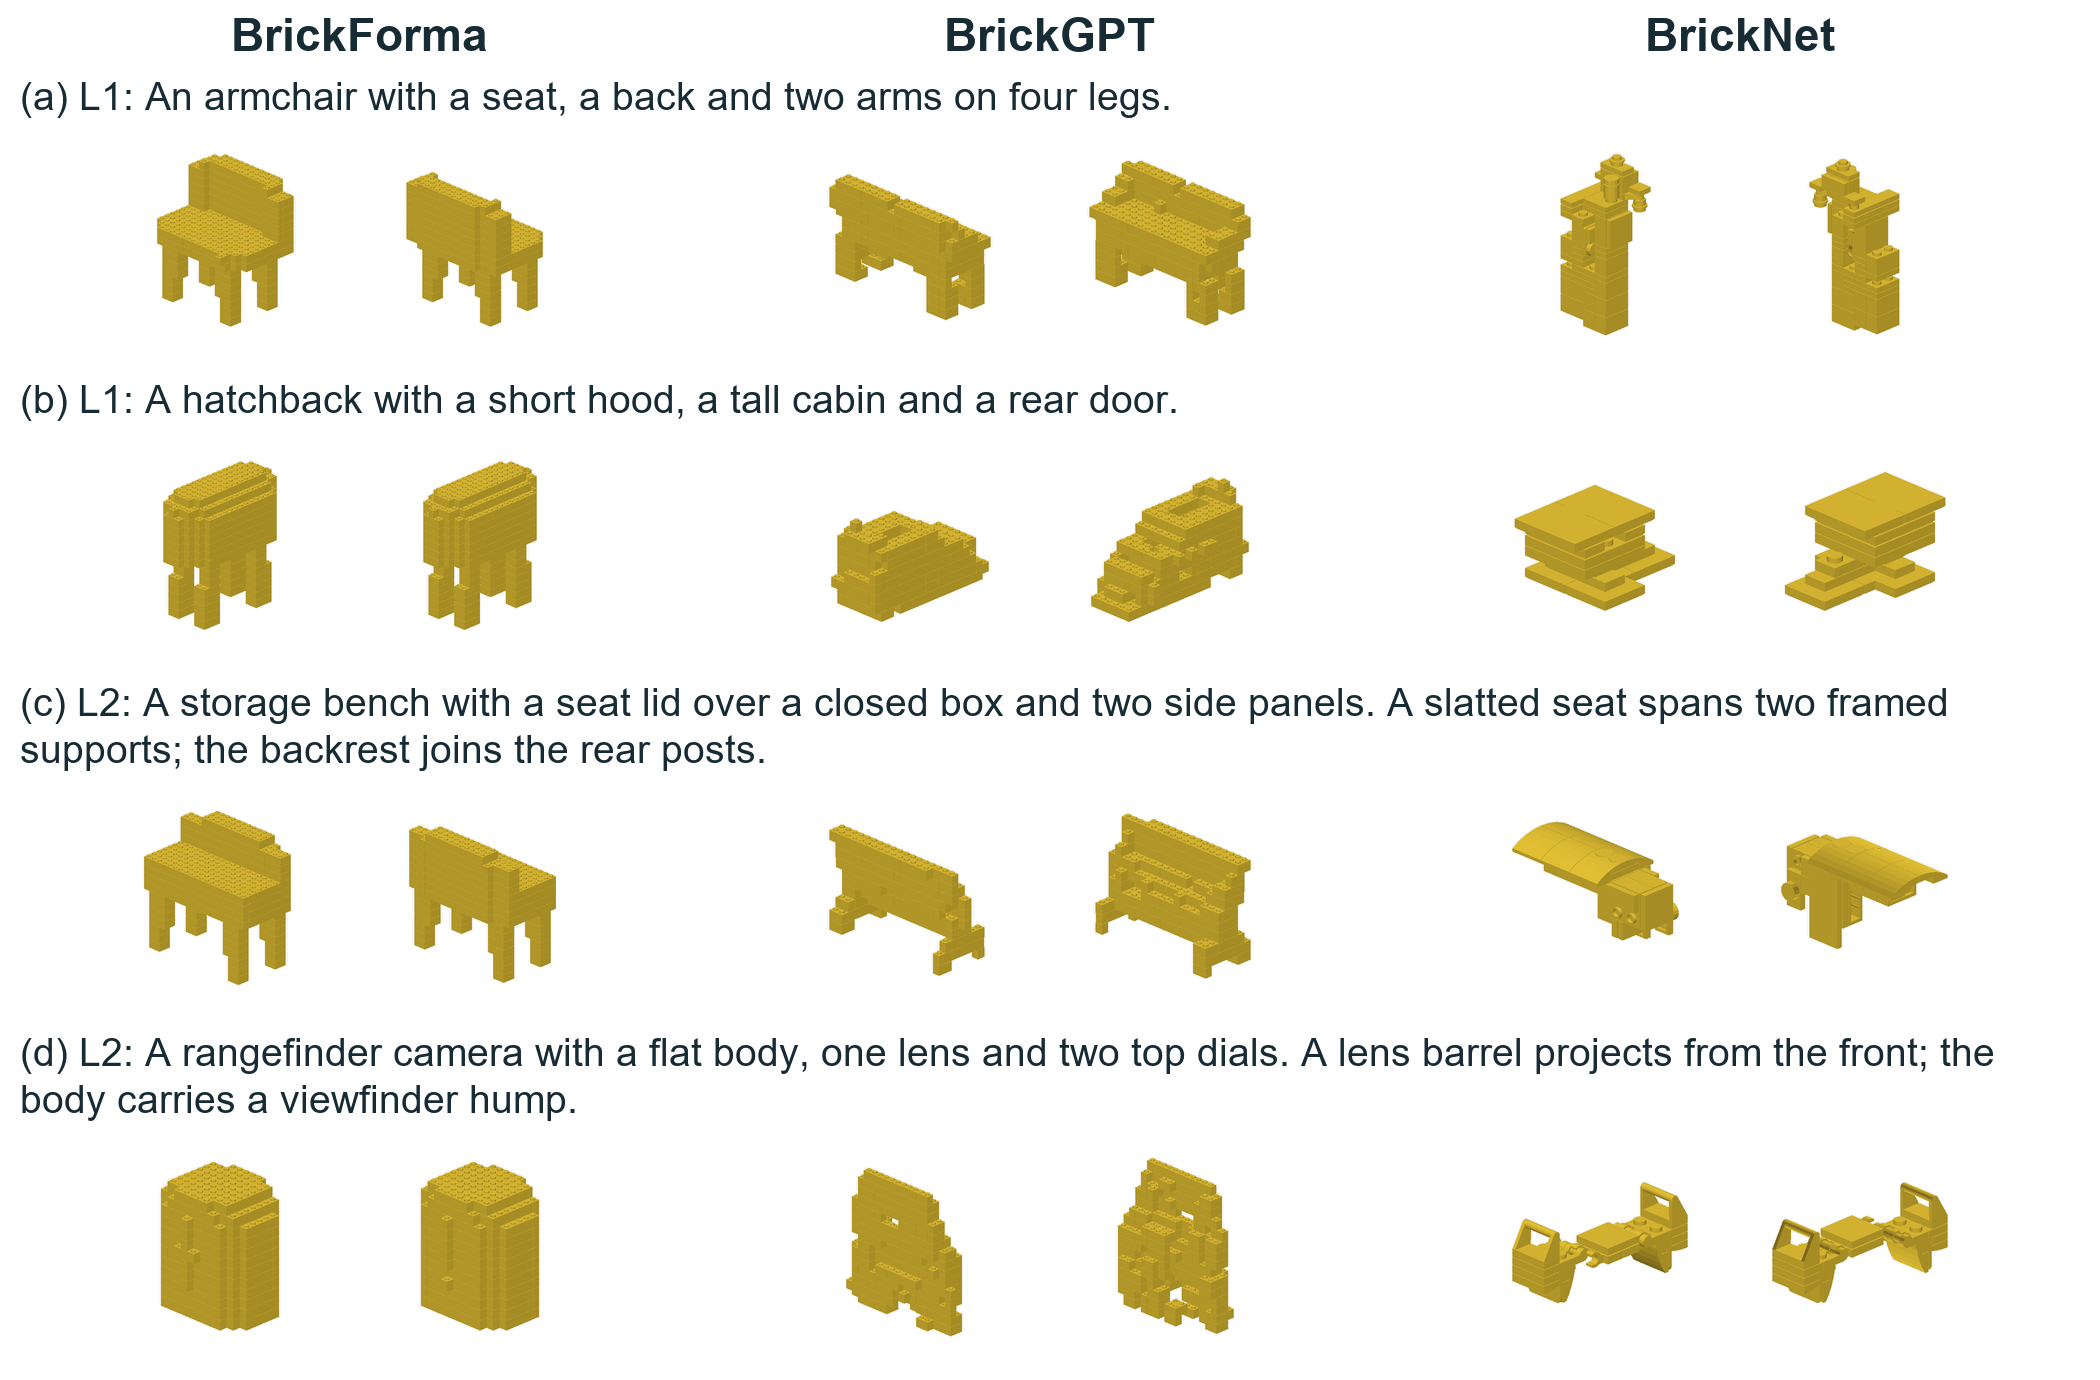
\includegraphics[width=\textwidth]{figures/matched_short_prompts_20261116.png}
\caption{Four examples from the matched evaluation with the same prompts, render settings, and azimuths ($45^\circ$ and $225^\circ$) across systems. The highest VQAScore belongs to BrickForma for the chair and bench, BrickGPT for the hatchback, and BrickNet for the camera.}
\label{fig:gallery}
\end{figure*}


\subsection{Raw versus Refined Outputs}
\begin{table}[t]
\centering
\small
\begin{tabular}{lrr}
\toprule
Metric & Raw & Refined \\
\midrule
$P_{\mathrm{inv}}$ $\downarrow$ & 0.1897\% & 0.0000\% \\
VQAScore $\uparrow$ & 0.2065 & 0.2071 \\
PE $\uparrow$ & 0.1858 & 0.1859 \\
SigLIP2 $\uparrow$ & 0.1379 & 0.1261 \\
Mean parts & 178.7 & 421.2 \\
\bottomrule
\end{tabular}
\caption{Earlier repair comparison on 110 pairs sharing the same prompt, model identifier, and caption.}
\label{tab:raw-refined}
\end{table}

We examine refinement on 110 raw/refined pairs from an earlier 114-prompt comparison (Table~\ref{tab:raw-refined}). Refinement reduces mean $P_{\mathrm{inv}}$ from 0.1897\% to 0.0000\% and increases mean part count from 178.7 to 421.2. VQAScore and PE change little, while SigLIP2 falls from 0.1379 to 0.1261. Each pair shares a prompt and model identifier.

\subsection{Geometric refinement Audit}
\label{sec:diagnostics}
We define stud contacts by footprint overlap across adjacent layers. We map the same 110 pairs to a grid with 20 LDU horizontal pitch and 24 LDU layer height and translate each export to a common occupied-cell origin. All 110 pairs have equal occupied voxel unions after translation. Single-component layouts rise from 18 to 110, and overlap-free layouts rise from 100 to 110 (Table~\ref{tab:export-audit}).
\begin{table}[t]
\centering\small
\begin{tabular}{@{}lrr@{}}
\toprule
Export measure & Raw & Refined \\
\midrule
Single stud component & 18/110 & 110/110 \\
Mean stud components & 4.29 & 1.00 \\
No body-cell overlap & 100/110 & 110/110 \\
\midrule
\multicolumn{3}{@{}l@{}}{Equal voxel unions after translation: 110/110} \\
\bottomrule
\end{tabular}
\caption{Earlier export audit of 110 matched raw/refined pairs. Union equality uses translation normalization.}
\label{tab:export-audit}
\end{table}


In the separate 525-prompt diagnostic run, 46 raw layouts have a single stud component. All 525 final layouts form one component and preserve their corresponding target unions after the reported recovery procedure (Appendix~\ref{app:eval}).

\subsection{Evaluation Boundaries}
The comparison uses delivered exports from systems with different inference settings and part libraries. The description levels vary in both content and length. PE truncates 121 prompts and SigLIP2 truncates 209 (Appendix~\ref{app:eval}). Uniform yellow rendering evaluates shape and layout without assessing color fidelity. The paired refinement audit describes the delivered selected pairs. Its denominator excludes unsuccessful solver attempts.


\section{Limitations and Discussion}
The program-based transfer combines generator design, geometric validation, and supervised fine-tuning. Isolating the contribution of large-model authoring would require an alternative generator evaluated under a matched training budget.

The dataset release checks grounding and coverage, and refinement enforces a single stud-connected component. Mechanical stability and a feasible assembly order require separate measurements. The integrated release and the training run record their counts separately (Table~\ref{tab:training-data}).

\section{Conclusion}
BrickForma converts program-generated voxels into checked brick layouts and uses them to fine-tune Qwen3-1.7B. Its raw outputs lead all three alignment metrics in aggregate on 525 matched prompts, with a mean invalid-placement ratio of 0.79\%. In the earlier paired audit, exact-cover refinement restores stud connectivity while preserving the occupied voxel union.

\bibliography{references}
\FloatBarrier
\appendix
\section{Technical Appendix: Dataset Details}
\label{app:dataset}
The historical figures and tables in this appendix retain the supplied measurements and model renders, with labels translated into English. They use release-specific versions and criteria and are not substitutes for the integrated statistics or the current main comparison.

\paragraph{Contact-based gravity screening.}
We model 8\,mm stud spacing, 9.6\,mm brick height, and 1\,g per occupied stud-brick cell. Each overlapping stud contributes four vertical contact points at the corners of a square with half-width 0.25 stud. The horizontal ground can only provide compression at the corners of ground-level brick footprints inset by 0.05 stud. A linear program (LP) seeks vertical force balance and balance of the two gravity-induced moments for every brick. We verify the resulting contact forces against these equations. After the final assembly passes, the same check is applied to the bricks through each completed layer, bottom to top. Each stud-connected component of a prefix is checked independently on the unanchored ground.

\paragraph{Tipping margin and clutch demand.}
The tipping margin is the minimum signed inward distance from the horizontal center-of-mass projection to the edges of the convex hull of the ground contacts. We convert the margin from studs to meters and reject zero or negative margins within numerical tolerance. If the compression-only LP is infeasible after this check, a second LP permits tension at internal stud contacts. It minimizes the largest total tensile force across the four contact points of any single stud. We report this minimum required clutch force in newtons per stud. Actual clutch capacity is uncalibrated. A verified compression-only solution qualifies for a gravity-screening pass, while solutions requiring tensile support are recorded separately.

\emph{Caption example.} The five captions of one model share a prefix and add detail level by level. The L1 prompt is \textquotedblleft An oval birdhouse with curved roof, enclosed room and front entrance.\textquotedblright\ Its L5 description is: ``An oval birdhouse with curved roof, enclosed room and front entrance. The protective roof joins the walls; the circular front entrance reaches a real interior cavity. Curved substantial surfaces carry their continuously attached functional parts. Overall width is 1.15 times depth; height is 0.80 times width. Parts follow functional positions. Continuous red, tan, brown color regions distinguish the body and attachments. The front reveals functional parts; side and top views reveal depth, connections and layout.''

\begin{table}[!htbp]
\centering
\small
\setlength{\tabcolsep}{3pt}
\begin{tabular}{lrrr}
\toprule
Release & Passing & Added & Removed \\
\midrule
Strict v3 & 7,902 & -- & -- \\
Relaxed & 65,503 & 428,278 & 38,230 \\
Local refinement & 79,298 & 228,582 & 125 \\ %Xu
\bottomrule
\end{tabular}
\caption{Geometric pass counts of the 80,000 source models under successive conversion releases (relaxed: several grounded components allowed), with total voxels added and removed, as in the corresponding release reports.}
\label{tab:conversion}
\end{table}

\begin{figure*}[!htbp]
\centering
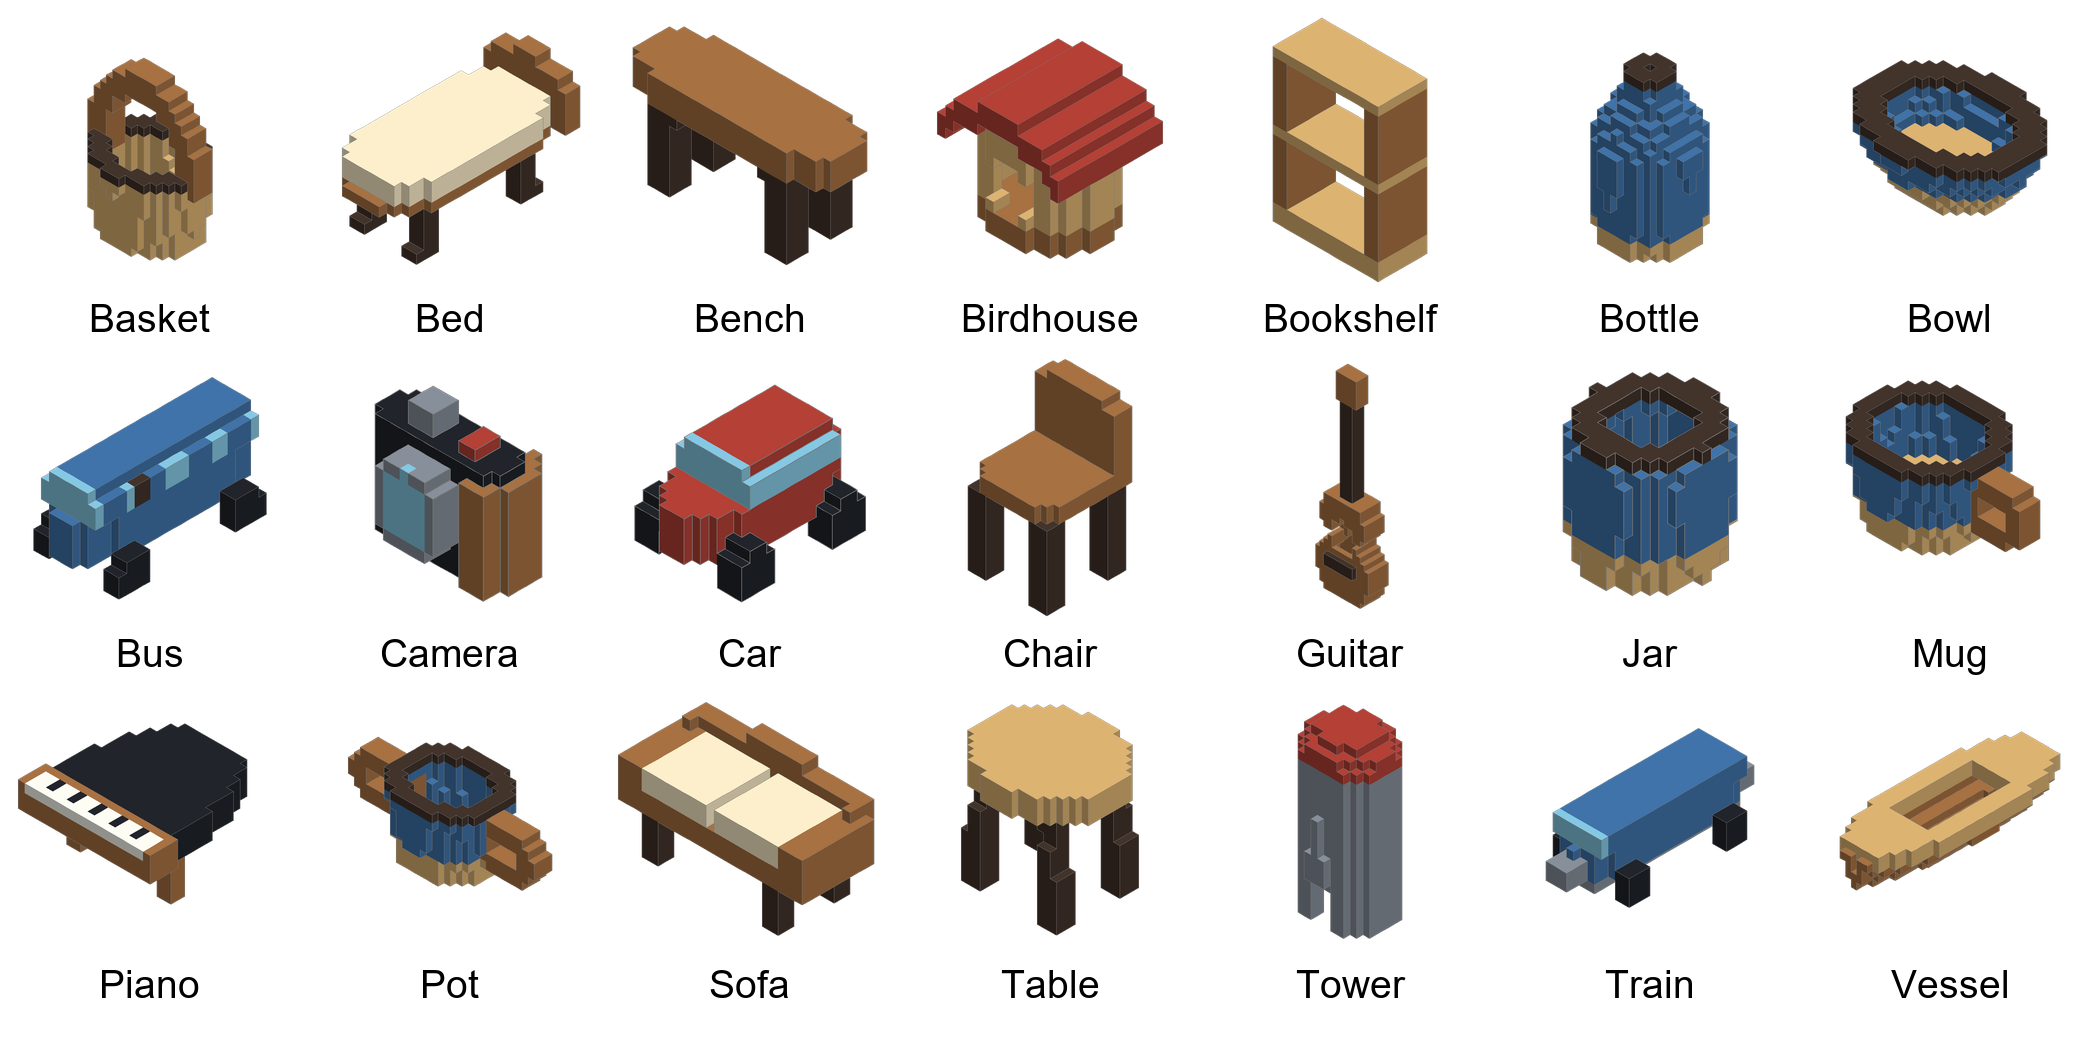
\includegraphics[width=\textwidth]{figures/image7_en.png}
\caption{Voxel model samples spanning the 21 object categories.}
\end{figure*}

\begin{figure*}[t]
\centering
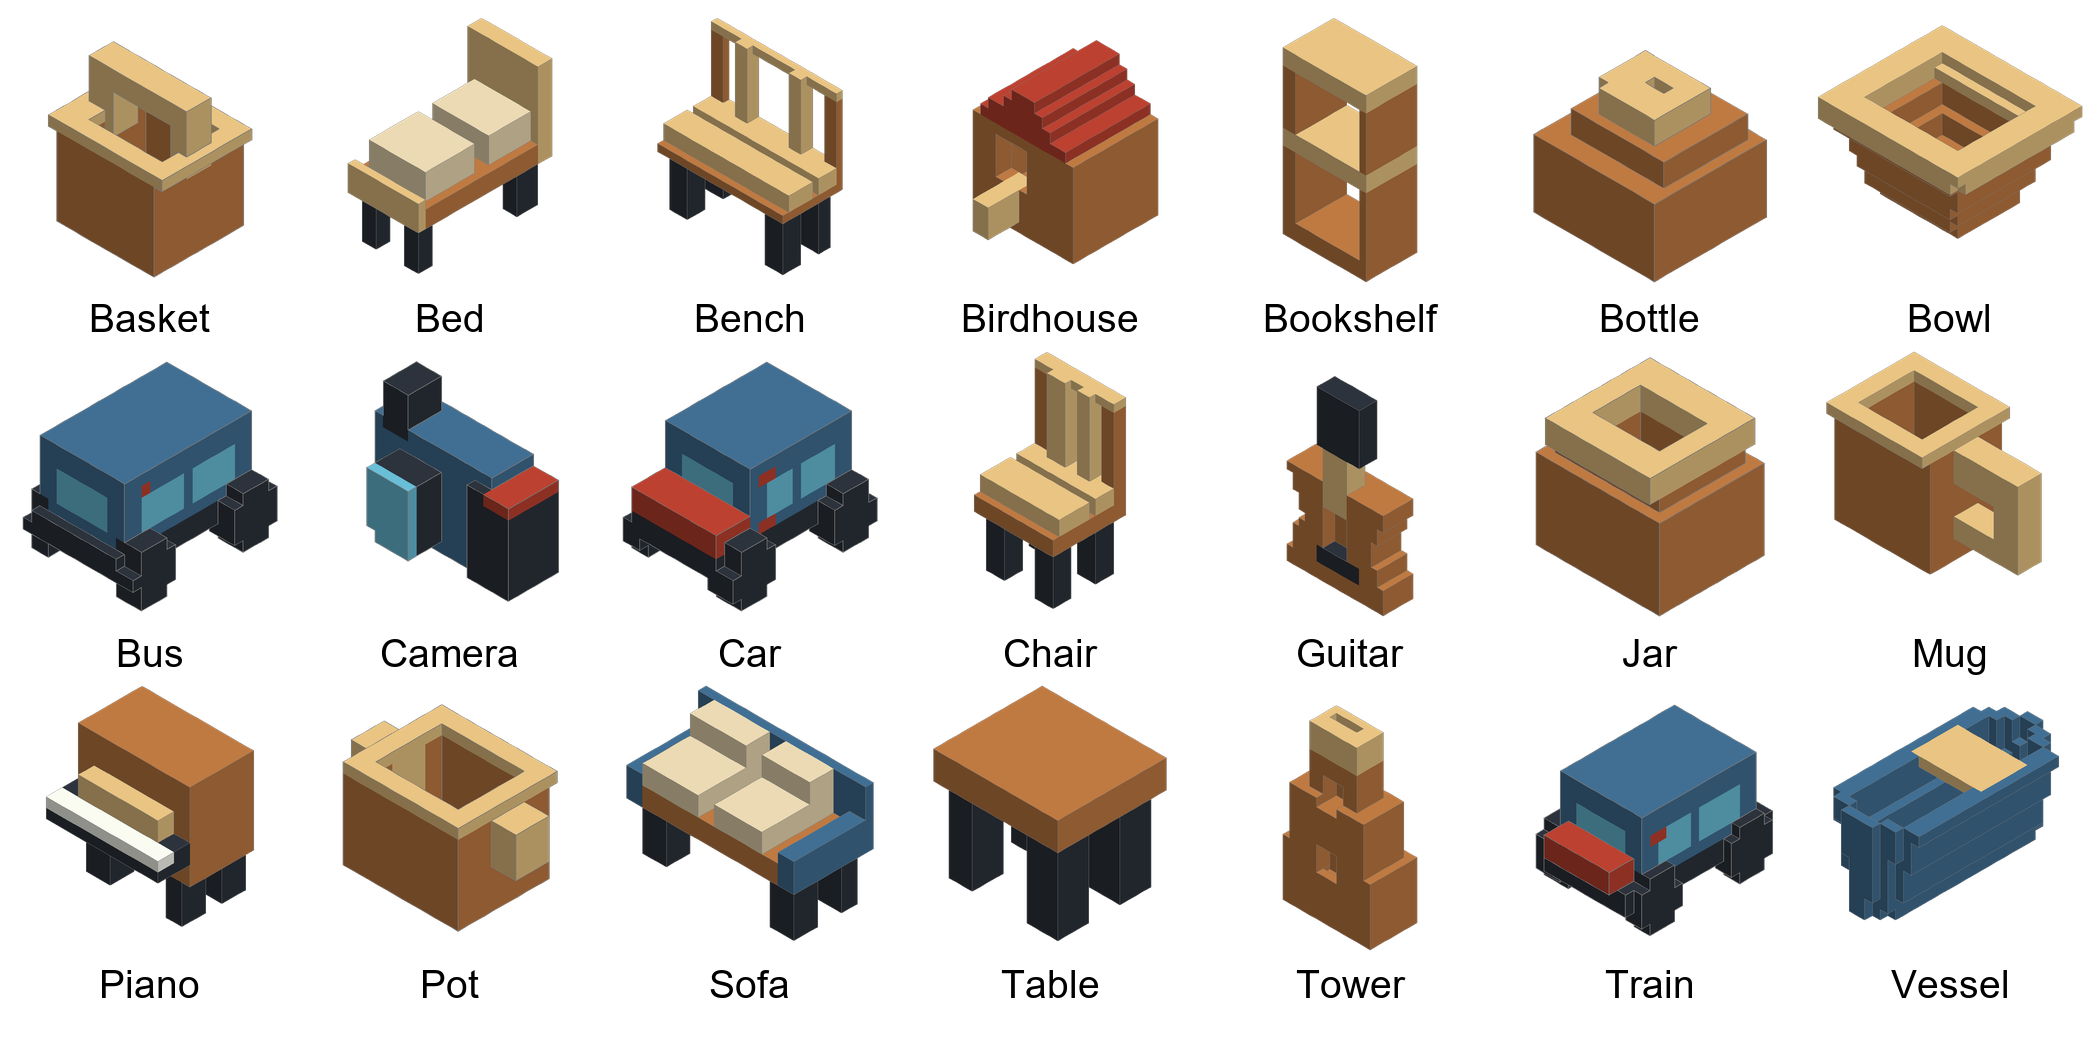
\includegraphics[width=\textwidth]{figures/image8_en.png}
\caption{Additional historical voxel model examples.}
\end{figure*}

\begin{figure*}[!htbp]
\centering
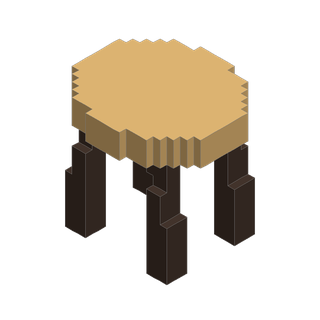
\includegraphics[width=0.118\textwidth]{figures/image4.png}\hfill
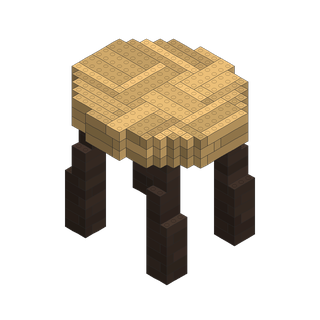
\includegraphics[width=0.118\textwidth]{figures/image5.png}\hfill
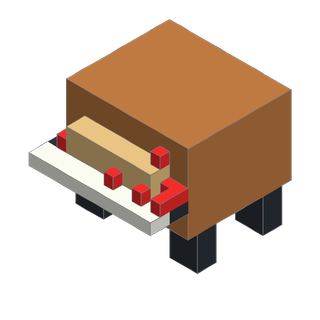
\includegraphics[width=0.118\textwidth]{figures/image2.png}\hfill
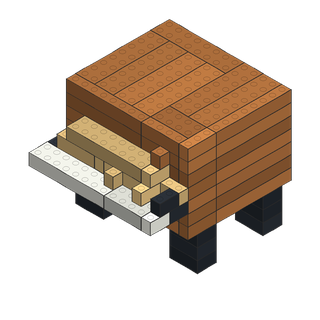
\includegraphics[width=0.118\textwidth]{figures/image3.png}\hfill
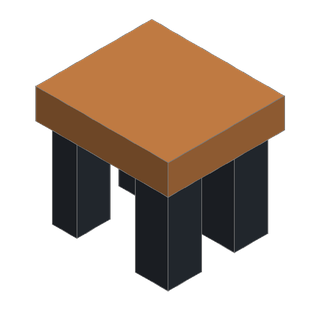
\includegraphics[width=0.118\textwidth]{figures/image9.png}\hfill
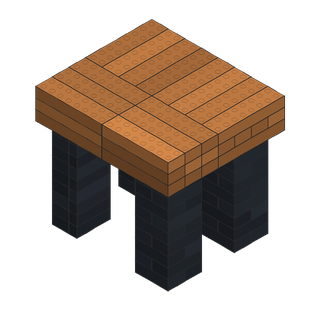
\includegraphics[width=0.118\textwidth]{figures/image10.png}\hfill

\includegraphics[width=0.118\textwidth]{figures/image11.png}\hfill
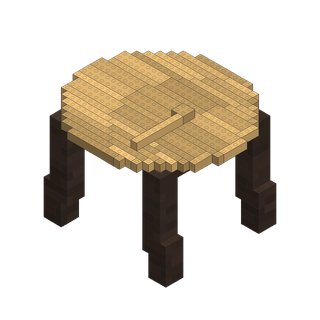
\includegraphics[width=0.118\textwidth]{figures/image12.png}
\caption{Historical examples of voxel targets and brick layouts after local repair.}
\end{figure*}

\begin{figure*}[t]
\centering
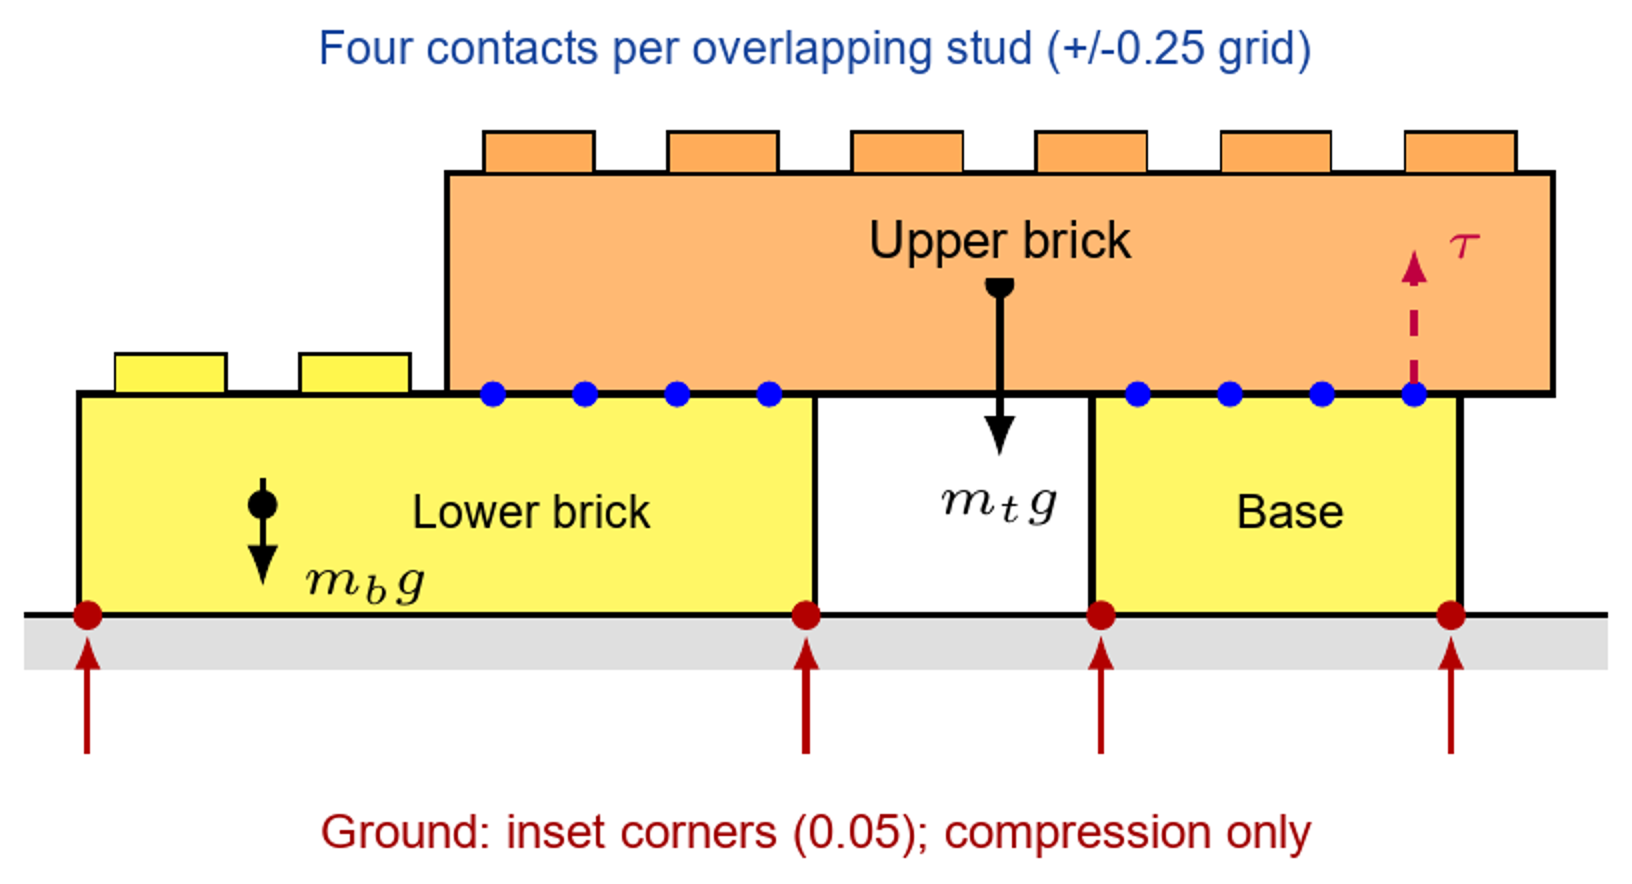
\includegraphics[width=0.75\textwidth]{figures/image13_en.png}
\caption{Historical contact-based gravity screening model, with English labels. The stated contact and ground assumptions are retained.}
\end{figure*}

\begin{figure*}[!htbp]
\centering
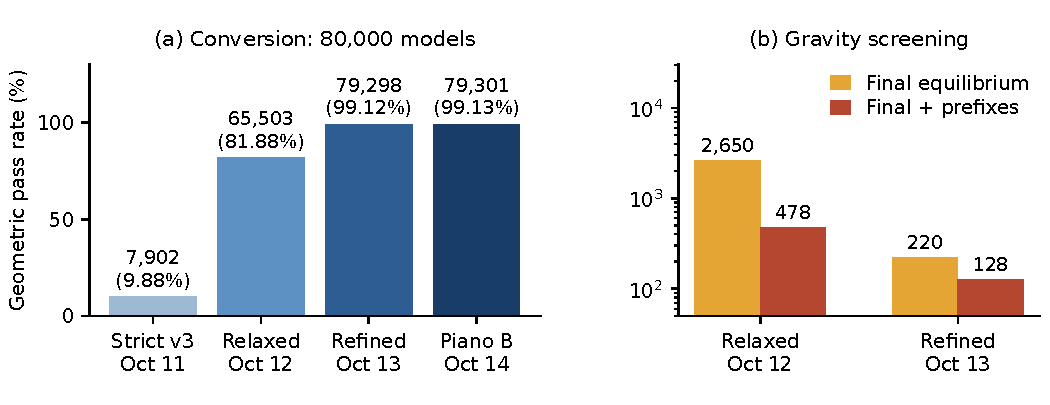
\includegraphics[width=\textwidth]{figures/image14_en.pdf}
\caption{Historical comparison of geometric conversion and screening outcomes across releases; values as in the corresponding release reports (Table~\ref{tab:conversion}).}
\end{figure*}

\begin{figure*}[!htbp]
\centering
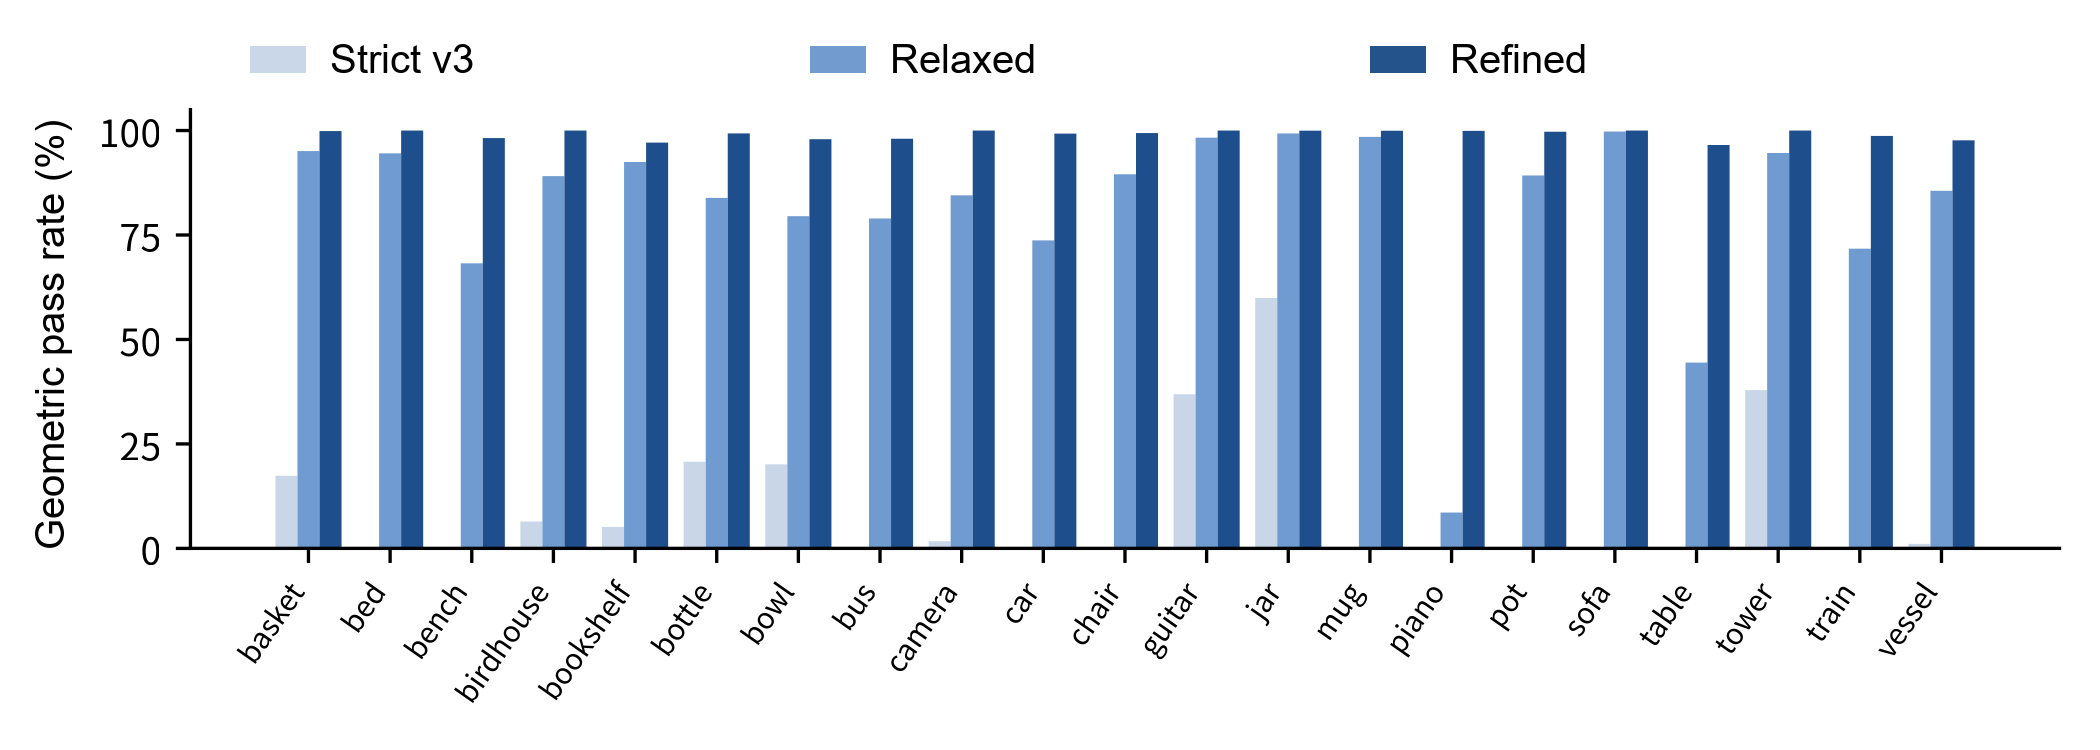
\includegraphics[width=\textwidth]{figures/image15_en.png}
\caption{Historical category-level geometric pass rates. Version and numerical labels require verification.}
\end{figure*}

\begin{figure*}[t]
\centering
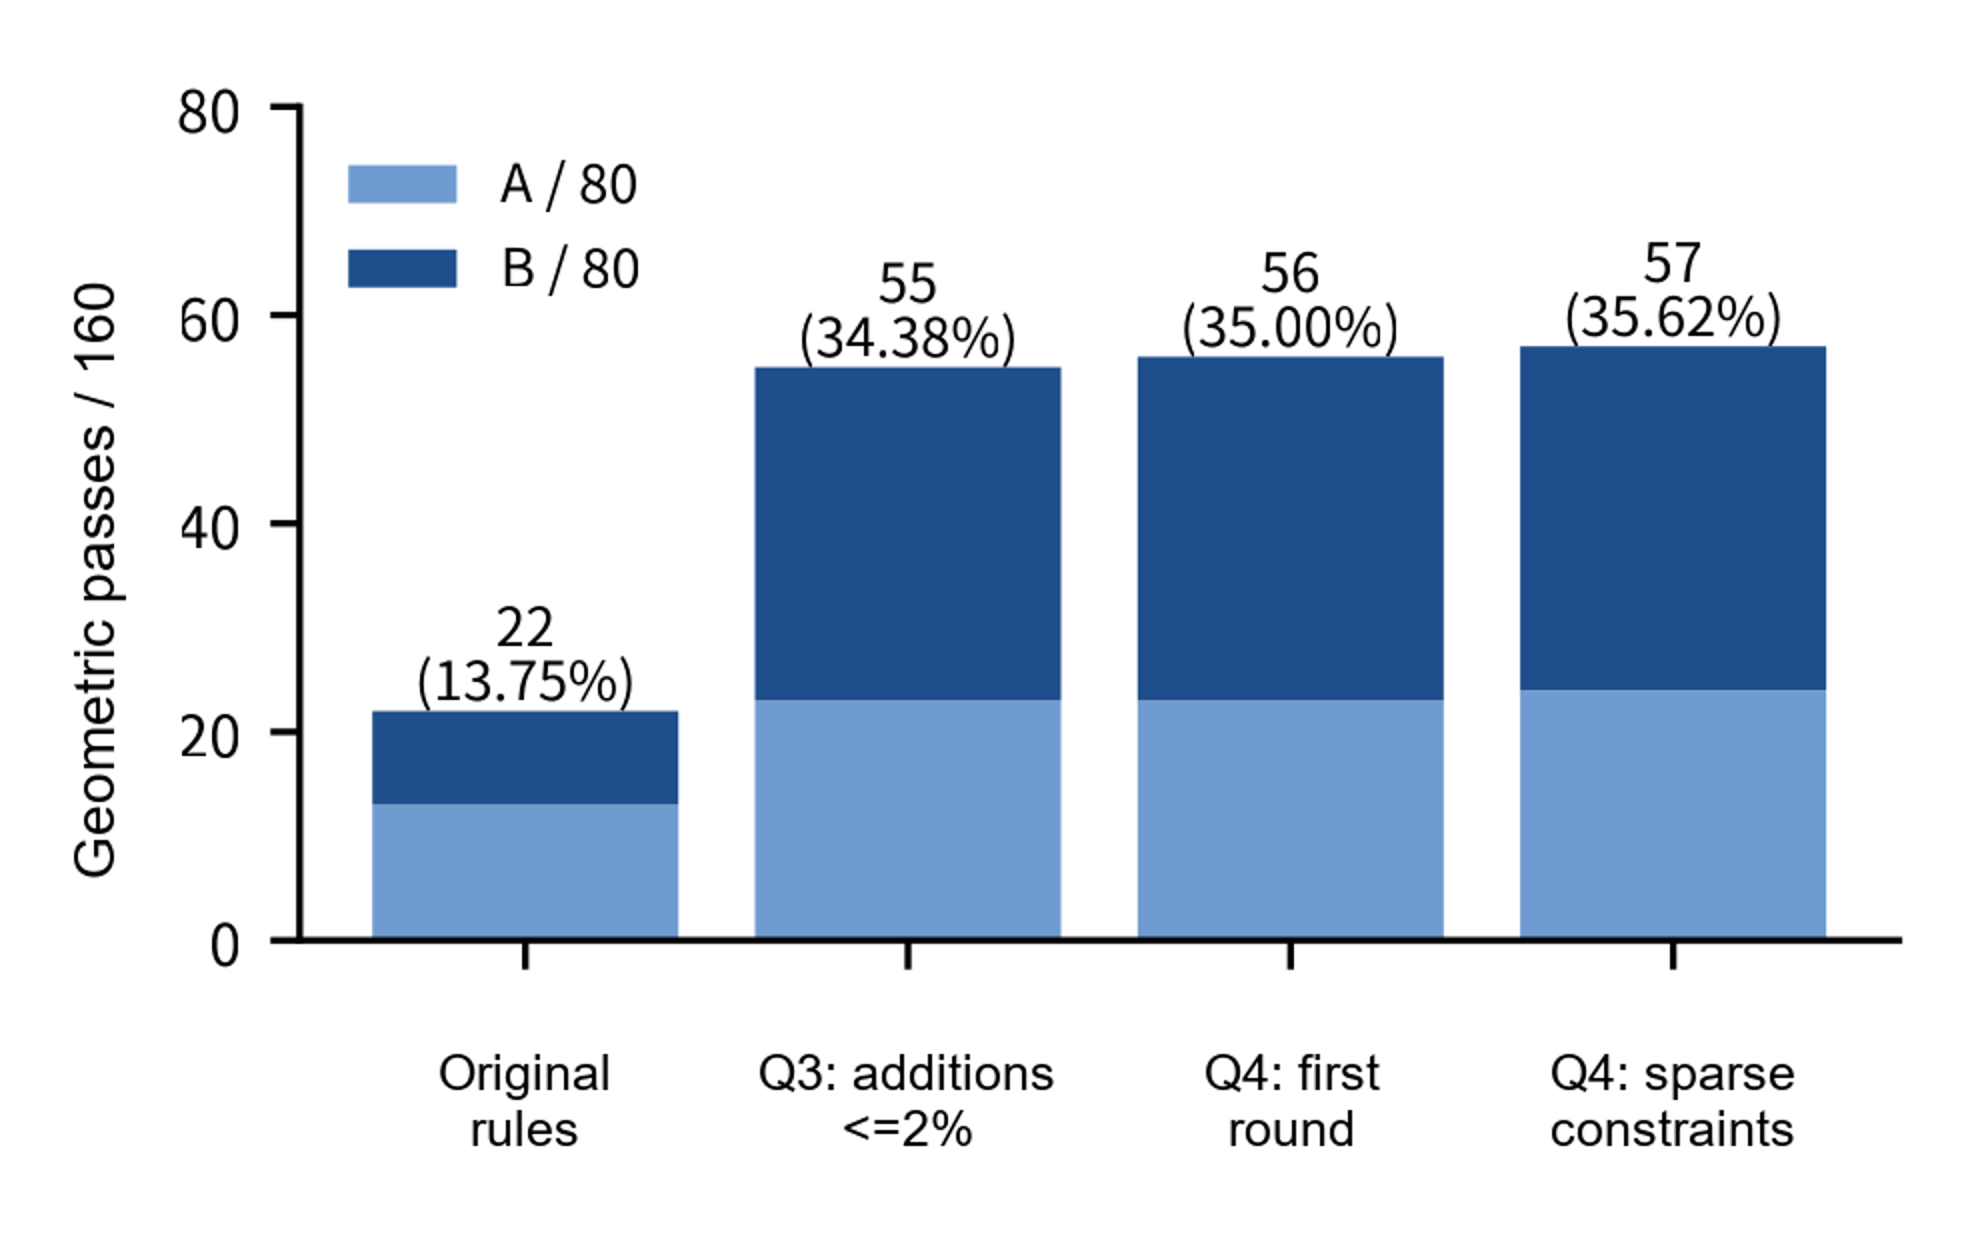
\includegraphics[width=0.72\textwidth]{figures/image16_en.png}
\caption{Historical results on a uniform 160-model sample. Version and numerical labels require verification.}
\end{figure*}

\begin{figure*}[!htbp]
\centering
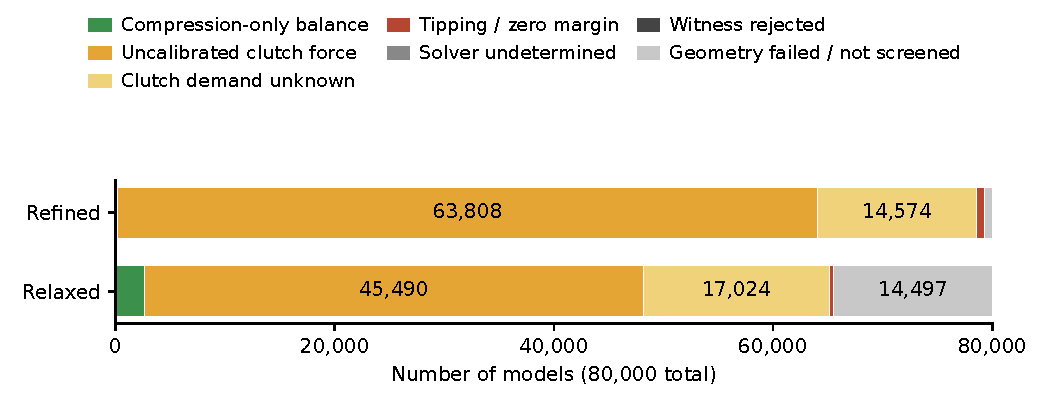
\includegraphics[width=\textwidth]{figures/image17_en.pdf}
\caption{Historical distributions of physical screening statuses; values as in the corresponding release reports. Counts refer to the specific releases shown and are kept separate from geometric pass rates.}
\end{figure*}


\section{Technical Appendix: Training Details}
\label{app:training}
Aggregate throughput is 24,448 tokens/s over eight GPUs, and the mean training loss is 0.0273. Evaluation and checkpointing run every 500 steps. With TRL~0.15, the unpacked multi-GPU path hangs after the first backward pass, which is why the TRL~0.17 stack is pinned. Because validation loss is lowest during epoch 2, two epochs would be a more economical setting for future runs (about one third less compute). The full software stack is transformers 4.51.3, trl 0.17.0, peft 0.15.2, datasets 3.6.0, and accelerate 1.6.0, with bf16 precision, gradient checkpointing, and unpacked sequences.

\begin{table}[!htbp]
\centering
\small
\begin{tabular}{lrr}
\toprule
Progress & Step & Validation loss \\
\midrule
Start & 500 & 0.1410 \\
--- & 1,500 & 0.0950 \\
--- & 10,500 & 0.0509 \\
--- & 22,500 & 0.0404 \\
$\approx$ End of epoch 1 & 44,500 & 0.0337 \\
--- & 65,500 & 0.0316 \\
Best (epoch 1.77) & 79,000 & 0.0308 \\
End of epoch 3 & 133,860 & 0.0339 \\
\bottomrule
\end{tabular}
\caption{Validation loss on the 2,000-sample validation subset. One epoch is $\approx$44,620 steps; the nearest evaluation to the end of epoch 1 is step 44,500.}
\label{tab:eval-loss}
\end{table}

% BrickGPT-paper column verified against arXiv:2505.05469 (Sec. 5.1 and Appendix A training details).
\begin{table*}[!htbp]
\centering
\small
\setlength{\tabcolsep}{5pt}
\begin{tabular}{lcc}
\toprule
Dimension & BrickGPT paper & Official Qwen3 script (ours) \\
\midrule
Base model & LLaMA-3.2-1B-Instruct & Qwen3-1.7B \\
LoRA & $r=32$, $\alpha=16$, dropout $0.05$, $q$/$v$ only (3.4M params) & $r=16$, $\alpha=32$, all linear layers \\
Learning rate & $2{\times}10^{-3}$ (AdamW) & $10^{-4}$ \\
Effective batch & 64 & 8 \\
Max length & 4,096 & 8,192 \\
Epochs & 3 & 3 \\
Hardware & 8$\times$RTX A6000, 12\,h & 8$\times$4090D, 25.3\,h \\
Data & StableText2Brick, 47k structures / 240k prompts & BrickForma-48, 79.3k models / 396,610 samples \\
\bottomrule
\end{tabular}
\caption{Our configuration versus the original BrickGPT paper \cite{brickgpt}. BrickGPT-paper values are taken from Sec.~5.1 and Appendix~A of arXiv:2505.05469 (base model, LoRA $r{=}32$, $\alpha{=}16$, dropout $0.05$, $q$/$v$ only with 3.4M parameters, AdamW learning rate $0.002$, global batch 64, 4096-token length filter, 3 epochs, 8$\times$RTX A6000 and 12\,h, and 47k+ structures / 240k prompts). The data organization, instruction template, absence of thinking mode, and LoRA paradigm follow BrickGPT; concrete hyperparameters follow the official Qwen3 adaptation, with the budget adjusted for the larger world, library, and corpus.}
\label{tab:brickgpt-recipe}
\end{table*}


\section{Technical Appendix: Additional Evaluation Material}
\label{app:eval}

\paragraph{Matched evaluation.}

The evaluation covers 1,575 exports and 12,600 rendered views. All four metrics are available for every export. We score every delivered raw BrickForma sequence, including drafts with incomplete generation or failed source geometry checks. Three supplied GLB previews contain only a prefix of the corresponding sequence. Scoring uses the delivered sequence in each case. BrickGPT uses a $20^3$ world and seed 42, with recorded regeneration budgets of 8 or 100 across its delivered exports.


\paragraph{Untuned Qwen3-1.7B.} We matched the base and fine-tuned runs by prompt text, category, and description level. Strict parsing found no placements for 178 of the 260 base outputs, and two used a part type outside the scoring catalog. The remaining 80 partial layouts and their raw BrickForma counterparts were scored with the same rendering and scorers. BrickForma scored higher on 78, 64, and 61 pairs for VQAScore, PE, and SigLIP2, respectively. The mean file-order invalid-placement ratios were 39.67\% for the parsed base layouts and 1.01\% for BrickForma. These rates depend on output completeness and recorded placement order. The paired scores are conditional on a scorable base layout and compare the delivered generation setups, which can differ in decoding.

\paragraph{Paired tests and truncation.}
Table~\ref{tab:sig} compares alignment scores on the 525 prompts. We use a two-sided exact sign test and a two-sided Wilcoxon signed-rank test with the normal approximation, excluding ties. Holm correction is applied separately to the six comparisons within each test. All adjusted $p$ values are below $2.0{\times}10^{-8}$. PE truncates 121 prompts and SigLIP2 truncates 209. On the untruncated subsets, BrickForma / BrickGPT / BrickNet score 0.1510 / 0.1408 / 0.1135 on PE (404 prompts) and 0.0340 / 0.0157 / 0.0009 on SigLIP2 (316 prompts).

\begin{table}[t]
\centering\small
\setlength{\tabcolsep}{3pt}
\begin{tabular}{llrrr}
\toprule
Baseline & Metric & W/L/T & Sign $p_H$ & Wilc.\ $p_H$ \\
\midrule
BrickGPT & VQAScore & 384/141/0 & $1.5\times 10^{-26}$ & $4.8\times 10^{-20}$ \\
 & PE & 337/188/0 & $1.6\times 10^{-10}$ & $3.1\times 10^{-12}$ \\
 & SigLIP2 & 327/198/0 & $2.0\times 10^{-8}$ & $7.3\times 10^{-12}$ \\
BrickNet & VQAScore & 460/65/0 & $1.6\times 10^{-73}$ & $4.6\times 10^{-60}$ \\
 & PE & 406/119/0 & $4.6\times 10^{-37}$ & $1.3\times 10^{-47}$ \\
 & SigLIP2 & 408/115/2 & $9.4\times 10^{-39}$ & $2.4\times 10^{-42}$ \\
\bottomrule
\end{tabular}
\caption{Two-sided paired tests on 525 prompts. W/L/T counts BrickForma wins, losses and ties. Each test uses Holm correction across six comparisons.}
\label{tab:sig}
\end{table}


\paragraph{Earlier 114-prompt comparison.} BrickGPT outputs were generated in its native $20^3$ world (seed 42), whereas BrickForma places bricks in a $48^3$ workspace, which partly explains the difference in part counts.
The systems differ in candidate selection, filtering, and post-processing.
On the BrickForma side, 45 of the 114 comparison outputs, together with their prompts, were chosen by human review as the best of six candidate phrasings in a category--level group; a winner was available in 79 of 105 groups, and 45 of those winners entered this comparison.
The remaining 69 outputs come from later fill-in, regeneration, colleague, and review rounds: 35 replaced a judged winner in 34 groups, and 34 filled 26 groups in which no candidate had been judged acceptable; together the 114 outputs cover all 105 groups.\footnote{The six candidates are the five new-batch phrasings and one first-batch phrasing documented in the evaluation-set README. Among the 69: \texttt{review\_59} 21, a colleague success set 16, second-round redo 12, third-round fill-in 7, colleague \texttt{nine\_ldr} 7, regeneration 5, and \texttt{car\_trials} 1, as recorded in the 11-07 delivery manifest. BrickGPT was then run once on each selected prompt (seed 42); BrickNet contributed one accepted sample per prompt (up to 30 attempts).}
The 114 outcomes comprised 110 refined layouts and four raw layouts. The earlier BrickGPT records report an eight-regeneration budget and Gurobi disabled.

\paragraph{Sensitivity of the earlier comparison.}
With equal weighting over the 105 category--level groups, BrickForma scores 0.2347 / 0.1840 / 0.1257 and BrickGPT scores 0.1511 / 0.1459 / 0.0318 on VQAScore / PE / SigLIP2. After excluding prompts truncated by each encoder, PE is 0.1821 versus 0.1445 on 89 prompts and SigLIP2 is 0.1088 versus 0.0301 on 85 prompts. The PE and SigLIP2 text encoders read at most 72 and 64 tokens, respectively.

\paragraph{Diagnostic cohort.}
To probe what the fine-tuned model learns, we inspected 525 BrickForma generations from a diagnostic set (21 categories $\times$ five levels $\times$ five phrasings). The 525-prompt diagnostic batch, together with 105 first-batch prompts, formed the six-phrasing candidate pool from which 45 of the 114 comparison outputs were selected (35 of them from the 525), as described above. Generation used seeds 42, 104, and 2026 in that order, moving to the next seed when a draft was incomplete or failed the geometry validator, then applied the 12--60--180\,s MILP ladder (the default loop of Algorithm~\ref{alg:inference-refinement}); raw drafts that already formed a single stud-connected component were kept unchanged. For 28 prompts a recovery path sampled seeds outside $S$; for two further prompts the solver budget was extended to 600\,s. Only 46 raw layouts (8.8\%) form a single stud-connected component without refinement; this rate shows no clear trend across levels (13, 9, 9, 7, and 8 for L1--L5) but varies strongly by category (e.g., 8/25 for sofa, 0/25 for basket and camera). All 479 failing raw layouts split into at least two stud components (median 5, maximum 33). Overlaps are a minor cause: 50 failing layouts contain duplicated voxels, 41 of them with at most five (median 2), and 429 contain none. The 2,240 detached fragments are mostly not grounded (1,320 airborne versus 920 grounded). The learned representation thus places bricks whose in-bounds voxel union is retained by refinement but that often fail to interlock across layers; all 525 final assemblies form a single stud-connected component with that union unchanged (Table~\ref{tab:diag} in Appendix~\ref{app:eval}). These checks evaluate stud connectivity and in-bounds voxel-union consistency, not prompt-level shape fidelity or spatial reasoning.

\begin{figure*}[t]
\centering
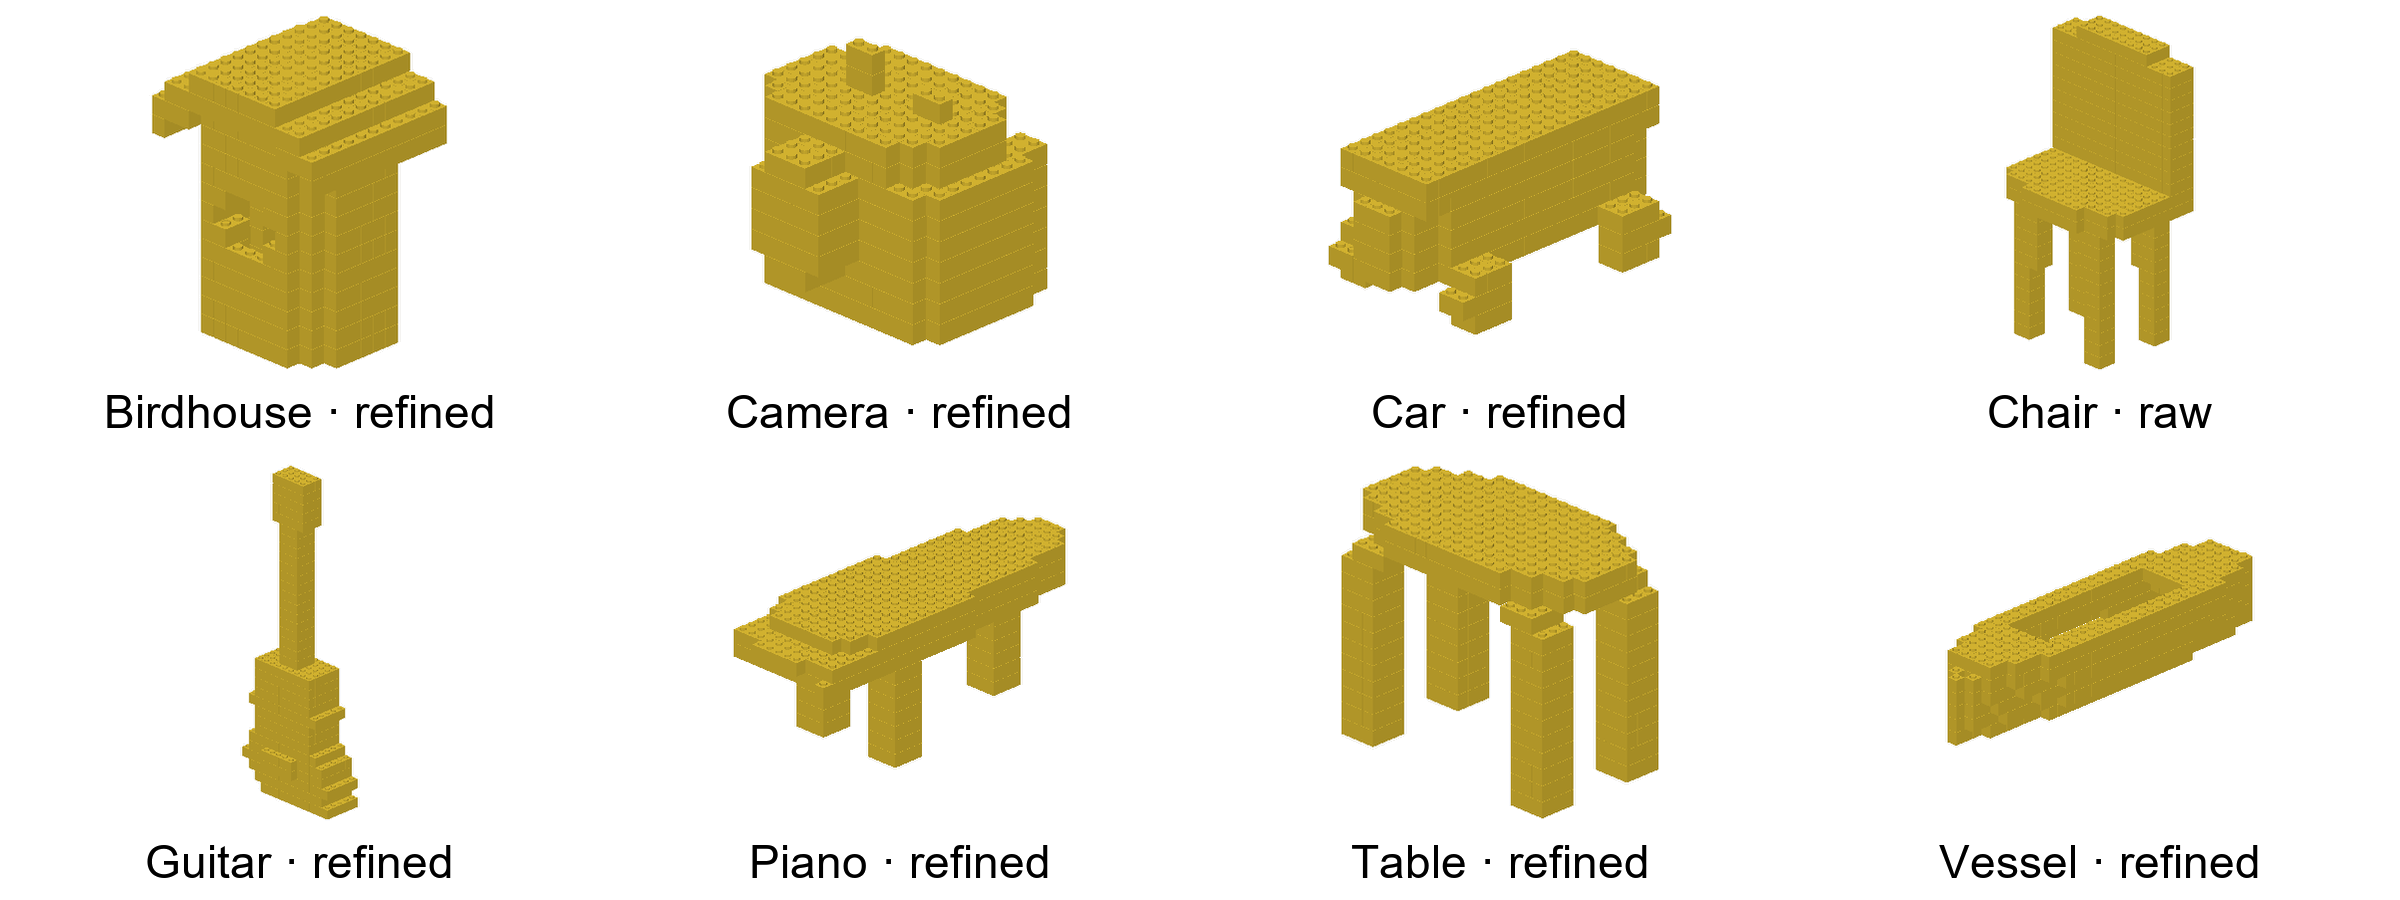
\includegraphics[width=\textwidth]{figures/generated_gallery_en.png}
\caption{BrickForma outputs from the earlier 114-prompt comparison. The chair is raw and the remaining examples are refined.}
\end{figure*}

\begin{table*}[!htbp]
\centering
\small
\setlength{\tabcolsep}{3pt}
\begin{tabular}{lr}
\toprule
Quantity (525 prompts) & Value \\
\midrule
Raw layout is a single stud component & 46 (8.8\%) \\
Stud components per failing raw (med./max) & 5 / 33 \\
Failing raw layouts with duplicated voxels & 50 / 479 \\
Detached fragments (airborne / grounded) & 1,320 / 920 \\
MILP tier reached (12 / 60 / 180 / 600\,s) & 326 / 133 / 18 / 2 \\
Prompts resampled outside $S$ & 28 \\
Final: single stud comp., union unchanged & 525 / 525 \\
Raw bricks, median (range) & 183 (77--623) \\
Final assembly bricks, median & 452 \\
\bottomrule
\end{tabular}
\caption{Structural diagnostics of raw outputs (Section~\ref{sec:diagnostics}). ``Union unchanged'' means the final assembly covers exactly the in-bounds voxel union of the raw draft; it does not assess whether the shape matches the prompt.}
\label{tab:diag}
\end{table*}



\begin{figure*}[!htbp]
\centering
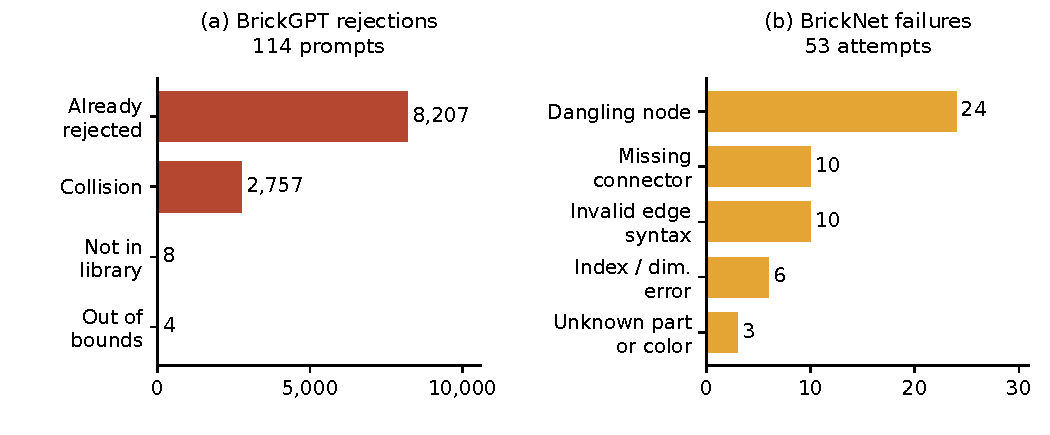
\includegraphics[width=\textwidth]{figures/image19_en.pdf}
\caption{Historical failure categories in the supplied reference; values as in the corresponding run records.}
\end{figure*}

\begin{figure*}[!htbp]
\centering
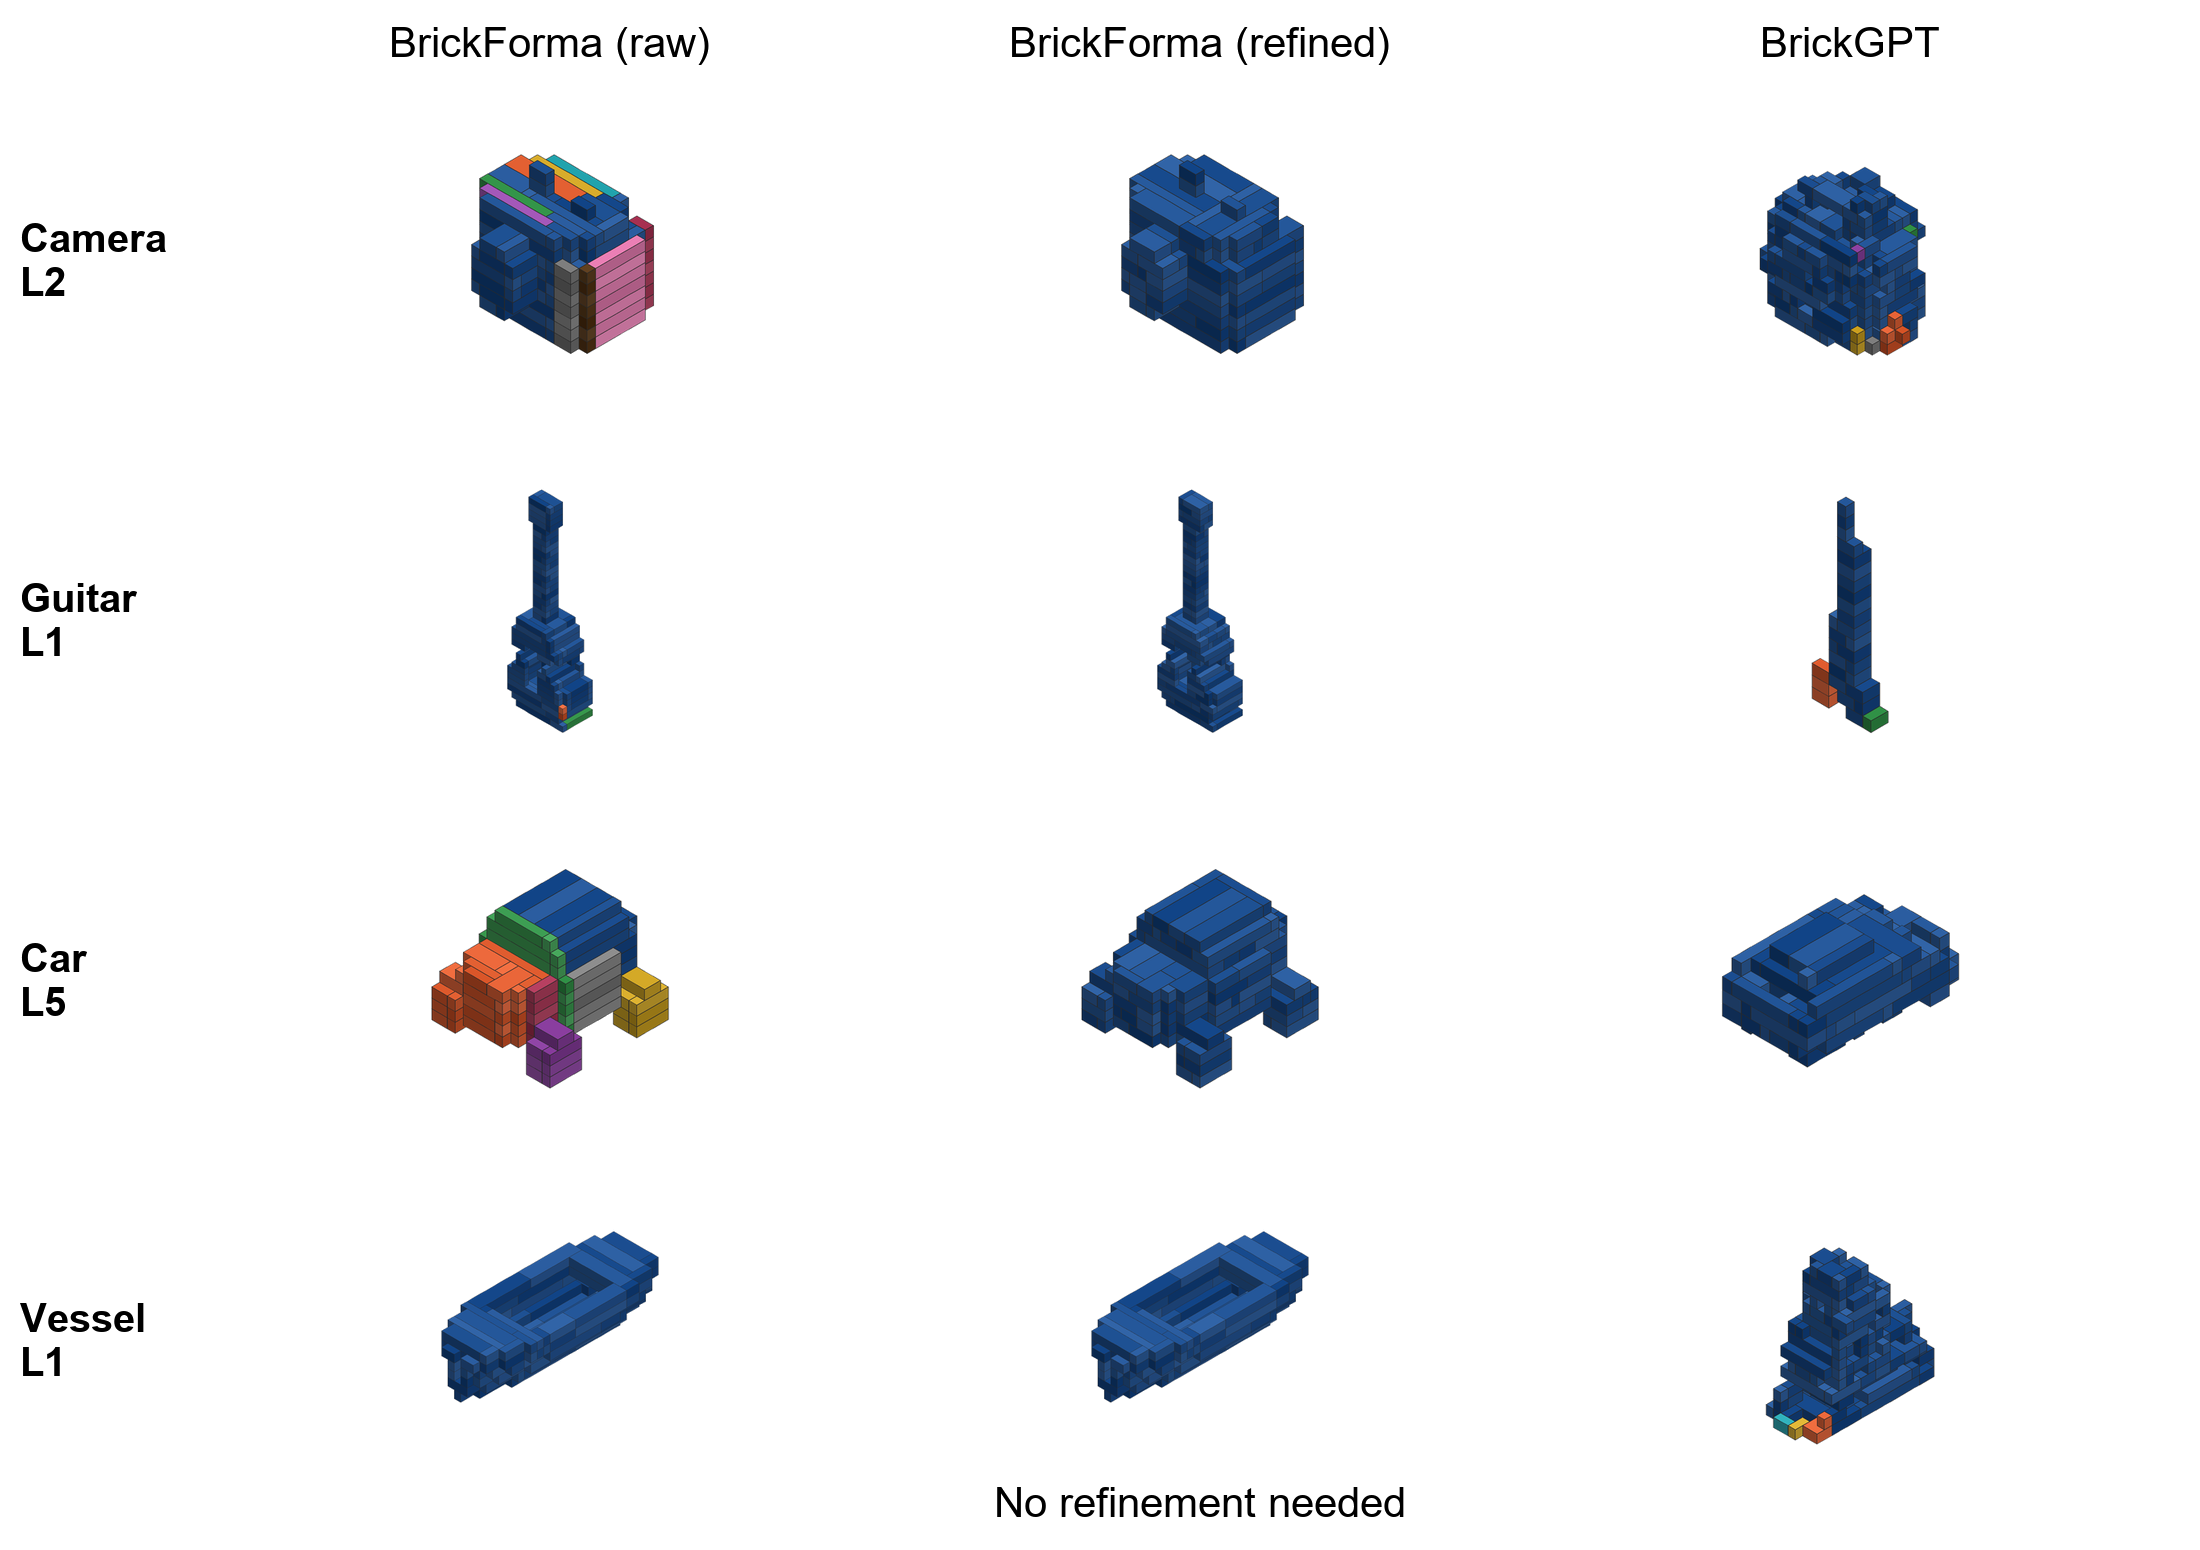
\includegraphics[width=\textwidth]{figures/original_comparison_en.png}
\caption{Qualitative historical examples from the supplied reference. Columns show raw and refined outputs of our system and BrickGPT outputs.}
\end{figure*}

\begin{figure*}[t]
\centering
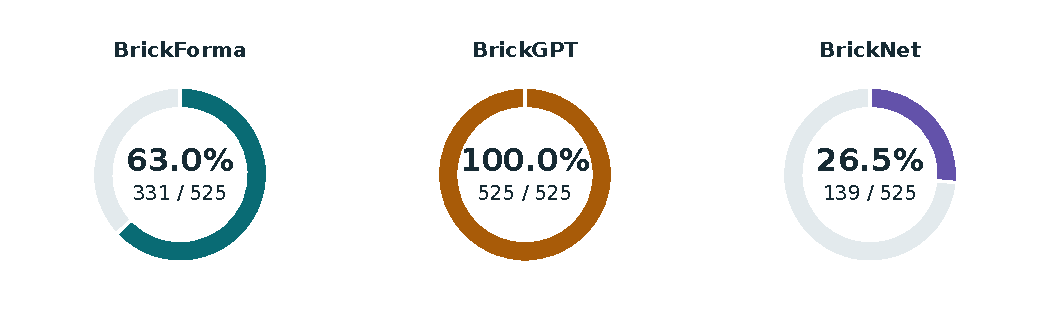
\includegraphics[width=\textwidth]{figures/comparison_20261117/01-zero-invalid.pdf}
\caption{Outputs with zero invalid placements on the 525 matched prompts. Colored arcs show $P_{\mathrm{inv}}=0$ and gray arcs show $P_{\mathrm{inv}}>0$. Each panel contains 525 outputs.}
\label{fig:comparison-zero-invalid}
\end{figure*}

\begin{figure*}[t]
\centering
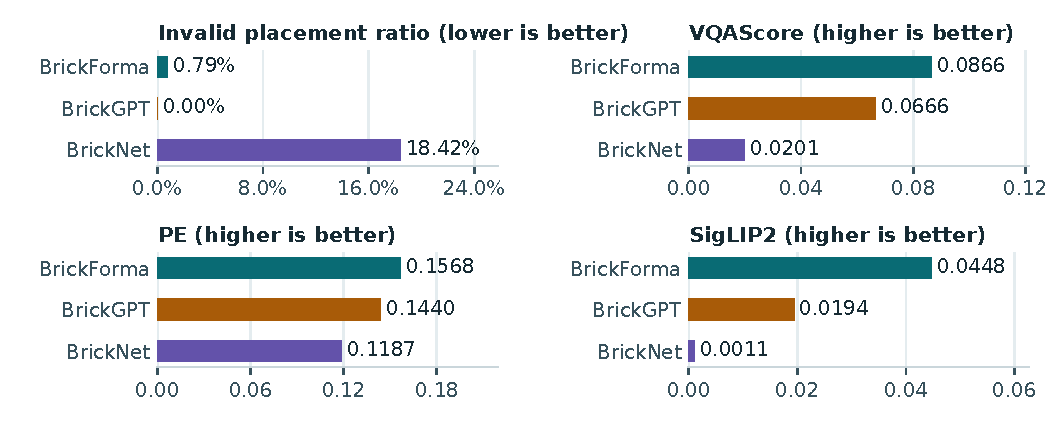
\includegraphics[width=\textwidth]{figures/comparison_20261117/02-means.pdf}
\caption{Mean scores on the 525 matched prompts. Each mean assigns equal weight to each prompt. The plotted values correspond to Table~\ref{tab:main}.}
\label{fig:comparison-means}
\end{figure*}

\begin{figure*}[t]
\centering
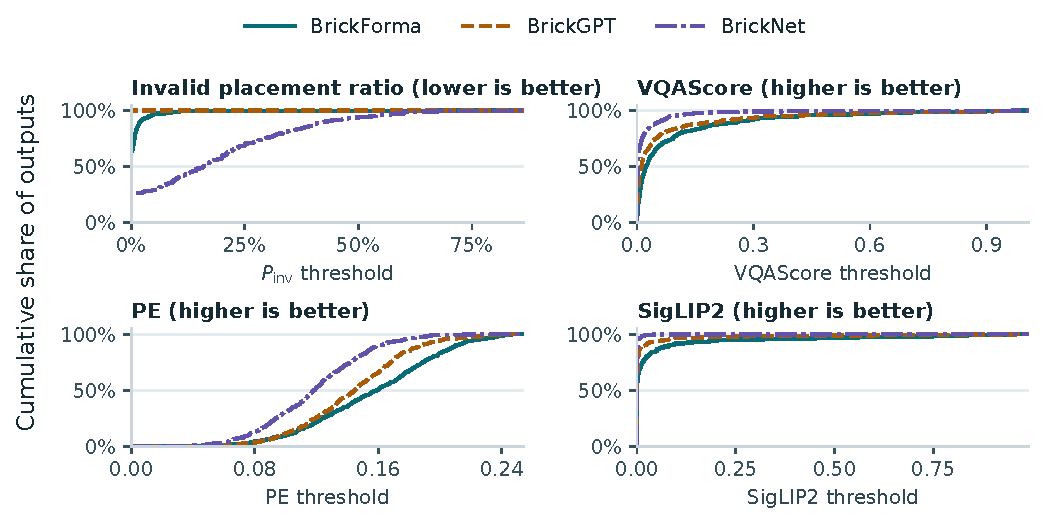
\includegraphics[width=\textwidth]{figures/comparison_20261117/03-distributions.pdf}
\caption{Empirical cumulative distributions of the four scores. Each curve gives the fraction of a system's 525 outputs at or below the threshold on the horizontal axis.}
\label{fig:comparison-distributions}
\end{figure*}

\begin{figure*}[t]
\centering
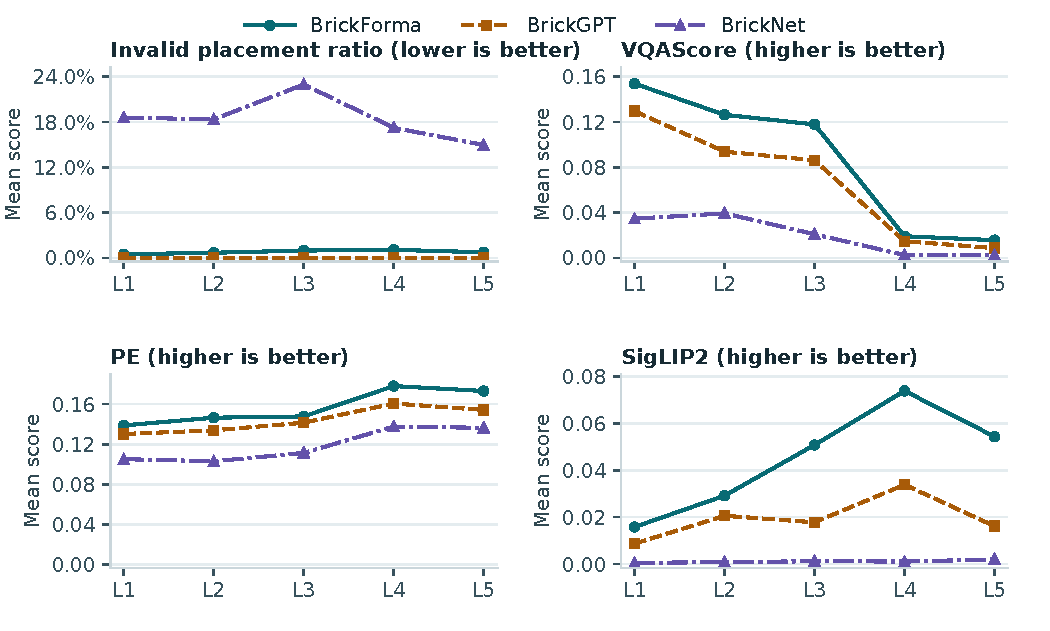
\includegraphics[width=\textwidth]{figures/comparison_20261117/04-by-level.pdf}
\caption{Mean scores from L1 to L5. Each point averages 105 prompts shared by all three systems (Table~\ref{tab:level-results}). From L3 to L4, VQAScore falls for all three systems while PE rises.}
\label{fig:comparison-levels}
\end{figure*}


\section{Technical Appendix: Historical Tables}
\label{app:historical}
The following transcribed tables preserve the historical reference material. They use different versions or evaluation criteria and are not substitutes for the current main comparison. Where a value is superseded by a verified number in the main text (e.g., Table~\ref{tab:training-data} and Appendix~\ref{app:dataset}), the main text takes precedence. Dashes indicate missing entries in the supplied source.
\begin{table*}[!htbp]\centering\small
\begin{tabular}{lr}\toprule
Item & Historical value \\ \midrule
Voxel models & 80,000 (40,000 per batch) \\
Categories / structural families & 21 / 40 per category \\
Grid / voxel count & $48^3$ / 750--1,250 \\
Prompt records & 400,000 (five bilingual records per model) \\
Uniqueness & 80,000 unique; 0 A/B duplicates \\
Overlap with historical hashes & 0 / 55,255 \\
Refined geometry passes & 79,298 (99.12\%) \\
Bricks in full preview & 12,718,389 \\
Final gravity equilibrium passes & 220 \\
Final and layer-prefix passes & 128 \\
\bottomrule\end{tabular}
\caption{Historical dataset statistics transcribed from the supplied reference. The geometry count refers to the old refined release, not the later integrated count. Verify the preview and physical-screening totals against version-matched reports.}
\end{table*}

\begin{table*}[!htbp]\centering\small
\setlength{\tabcolsep}{3pt}
\begin{tabular}{@{}l>{\raggedright\arraybackslash}p{3.9cm}>{\raggedright\arraybackslash}p{2.5cm}rrrr@{}}\toprule
Version & Connectivity & Voxel changes & Passes & Rate & Final & Both \\ \midrule
Strict v3 & Single; support $\geq$10\%, overhang $\leq$2 & None & 7,902 & 9.88\% & -- & -- \\
Relaxed & Each component grounded & +428,278 / -38,230 & 65,503 & 81.88\% & 2,650 & 478 \\
Refined & Each component grounded & +228,582 / -125 & 79,298 & 99.12\% & 220 & 128 \\
\midrule
\multicolumn{7}{l}{Uniform 160-model sample (seed 38177); not full-dataset results} \\
Baseline & Single stud-connected component & None & 22 & 13.75\% & -- & -- \\
Q3 & Single stud-connected component & Added $\leq$2\% & 55 & 34.38\% & 8 & 2 \\
Q4 (sparse) & Single stud-connected component & Added + removed $\leq$2\% & 57 & 35.63\% & 8 & 2 \\
\bottomrule\end{tabular}
\caption{Historical conversion-strategy table from the reference. Full-dataset and 160-model sample rows use different scopes; connectivity rules also differ. Final and Both columns report final-equilibrium and final-plus-prefix screening passes under the stated historical assumptions.}
\end{table*}

\begin{table*}[!htbp]\centering\small
\begin{tabular}{lrrr}\toprule
Item & BrickGPT & BrickNet 1.7B & BrickForma-48 \\ \midrule
Representation & $20^3$ bricks & Assembly graph & $48^3$ bricks \\
Criterion & stable & Parseable & -- \\
Passes & 66/114 & 114/114 & -- \\
Median parts & 126.5 & 22 & -- \\
Range & 19--497 & 6--48 & -- \\
Mean time (s) & 189.6 & -- & -- \\
\bottomrule\end{tabular}
\caption{Historical baseline table in the source reference. These criteria differ, and missing BrickForma-48 entries were marked TODO. This is not the current matched four-metric main table.}
\end{table*}

\begin{table*}[!htbp]\centering\small
\begin{tabular}{lrrrrl}\toprule
Level & $n$ & BrickGPT stable & GPT median bricks & Net median parts & BrickForma-48 \\ \midrule
L1 & 21 & 13 & 112 & 15 & -- \\
L2 & 21 & 15 & 118 & 22 & -- \\
L3 & 23 & 12 & 102 & 22 & -- \\
L4 & 25 & 12 & 140 & 21 & -- \\
L5 & 24 & 14 & 150.5 & 29.5 & -- \\
\bottomrule\end{tabular}
\caption{Historical level-wise baseline table transcribed from the reference. The original BrickForma-48 column was incomplete, and the other columns use different criteria.}
\end{table*}

\begin{table*}[!htbp]\centering\small
\begin{tabular}{lrrrr}\toprule
Method and source & $P_{\mathrm{inv}}$ & VQA & PE & SigLIP2 \\ \midrule
BrickGPT (literature, as transcribed) & 0.063 & 0.050 & 0.157 & 0.052 \\
BrickNet 1.7B (literature, as transcribed) & 0.260 & 0.593 & 0.282 & 0.631 \\
BrickGPT (114 prompts, historical placeholder) & -- & -- & -- & -- \\
BrickNet (114 prompts, historical placeholder) & -- & -- & -- & -- \\
BrickForma-48 (114 prompts, historical placeholder) & -- & -- & -- & -- \\
\bottomrule\end{tabular}
\caption{Original reference table with literature values and historical placeholders. Literature values use another evaluation set and must not be directly compared with the current 525-prompt results; the precise $P_{\mathrm{inv}}$ definition and direction require checking against the original publication.}
\end{table*}


\end{document}
